%% ------------------------------------------------------------------------
% LaTeX - Preambel ******************************************************
% ------------------------------------------------------------------------
% Dokumentklasse (Koma Script)
% ------------------------------------------------------------------------
% basiernd auf www.matthiaspospiech.de/latex/vorlagen Diplomarbeit kompakt
% ========================================================================
\documentclass[%
   %draft,            % Entwurfsstadium
   final,             % fertiges Dokument
   11pt,              % Schriftgroesse der Grundschrift
   bigheadings,       % gro�e �berschriften
   ngerman,           % wird an andere Pakete weitergereicht
   a4paper,           % Papierformat
   BCOR5mm,          % Bindekorrektur: Zus�tzlicher Rand auf der Innenseite
   DIV14,            % Seitengr��e (siehe Koma Skript Dokumentation !)
   1.1headlines,     % Zeilenanzahl der Kopfzeilen
   pagesize,         % Schreibt die Papiergroesse in die Datei.
   oneside,          % Einseitiges Layout
%   twoside,          % Zweiseitiges Layout
   openright,        % Kapitel beginnen immer auf der rechten Seite
   titlepage,        % Titel als einzelne Seite ('titlepage' Umgebung)  
   headsepline,      % Linie unter Kolumnentitel ()
%   plainheadsepline, % Linie unter Kolumnentitel () plain Seitenstil
   nochapterprefix,  % keine Ausgabe von 'Kapitel:'
   bibtotoc,         % Bibliographie ins TOC
%	bibtotocnumbered, % Bibliographie ins TOC mit Kapitelnummer
   tocindent,        % eingereuckte Gliederung
   listsindent,      % eingereuckte LOT, LOF
   pointlessnumbers, % �berschriftnummerierung ohne Punkt, siehe DUDEN !
   cleardoubleempty, % Leere linke Seite bei Zweiseitenlayout vor Kapitel
   fleqn,            % Formeln werden linksbuendig angezeigt
%   parindent,        % Absatz mit Einzug (Standard)
   halfparskip,      % Absatz halbe Zeile Abstand
%   parskip,          % Absatz ganze Zeile Abstand
]{scrbook}%     Klassen: scrartcl, scrreprt, scrbook

%% ------------------------------------------------------------------------
% LaTeX - Preambel ******************************************************
% ------------------------------------------------------------------------
% Packages
% ------------------------------------------------------------------------
% basiernd auf www.matthiaspospiech.de/latex/vorlagen Diplomarbeit kompakt
% ========================================================================

% Inhalt:
% 1. Einige Pakete muessen unbedingt vor allen anderen geladen werden
% 2. Fonts Fonts Fonts
% 3. Math Packages
% 4. Symbole
% 5. text related packages
% 6. Pakete zum Zitieren
% 7. PDF related packages
% 8. Tables (Tabular)
% 9. figures and placement
% 10. verbatim packages
% 11. science packages
% 12. layout packages

% ~~~~~~~~~~~~~~~~~~~~~~~~~~~~~~~~~~~~~~~~~~~~~~~~~~~~~~~~~~~~~~~~~~~~~~~~
% Encoding der Dateien (sonst funktionieren Umlaute nicht)
% Empfohlen latin1, da einige Pakete mit utf8 Zeichen nicht
% funktionieren, z.B: listings, soul.

\usepackage[latin1]{inputenx} % ISO-8859-1
%\usepackage[ansinew]{inputenx} % Windows-Standard (CP1252) (baut auf ISO 8859-1 und ISO 8859-15 auf)
%\usepackage[utf8]{inputenc}

% ~~~~~~~~~~~~~~~~~~~~~~~~~~~~~~~~~~~~~~~~~~~~~~~~~~~~~~~~~~~~~~~~~~~~~~~~
% 1. Einige Pakete muessen unbedingt vor allen anderen geladen werden
% ~~~~~~~~~~~~~~~~~~~~~~~~~~~~~~~~~~~~~~~~~~~~~~~~~~~~~~~~~~~~~~~~~~~~~~~~
%
\usepackage{xspace} % Define commands that don't eat spaces.
\usepackage{ifpdf} % Fuer Pakete/Paketoptionen, die nur fuer pdf benoetigt werden \ifpdf \else \fi
\usepackage{calc} % Calculation with LaTeX
\usepackage[ngerman]{babel} % Languagesetting
\usepackage[table]{xcolor} % Farben
\usepackage[]{graphicx} % Bilder
%\usepackage{epstopdf} % If an eps image is detected, epstopdf is automatically called to convert it to pdf format.
\usepackage[]{amsmath} % Amsmath - Mathematik Basispaket
\usepackage{ragged2e} % Besserer Flatternsatz (Linksbuendig, statt Blocksatz)

% ~~~~~~~~~~~~~~~~~~~~~~~~~~~~~~~~~~~~~~~~~~~~~~~~~~~~~~~~~~~~~~~~~~~~~~~~
% 2. Fonts Fonts Fonts
% ~~~~~~~~~~~~~~~~~~~~~~~~~~~~~~~~~~~~~~~~~~~~~~~~~~~~~~~~~~~~~~~~~~~~~~~~

\usepackage[T1]{fontenc} % T1 Schrift Encoding (notwendig f�r die meisten Type 1 Schriften)
\usepackage{textcomp}	 % Zusatzliche Symbole (Text Companion font extension)

% Alle Schriften die hier angegeben sind sehen im PDF richtig aus.
% Die LaTeX Standardschrift ist die Latin Modern (lmodern Paket).
% If Latin Modern is not available for your distribution you must install the
% package cm-super instead. Otherwise your fonts will look horrible in the PDF

% DO NOT LOAD ae-Package for the font !

%% - Latin Modern
\usepackage{lmodern}
%% -------------------
%
% % - Times, Helvetica, Courier (Word Standard...)
%\usepackage{mathptmx}
%\usepackage[scaled=.90]{helvet}
%\usepackage{courier}
% % -------------------
%%
%% - Palantino , Helvetica, Courier
%\usepackage{mathpazo}
%\usepackage[scaled=.95]{helvet}
%\usepackage{courier}
%% -------------------
%
%% - Bera Schriften
%\usepackage{bera}
%% -------------------
%
%% - Charter, Bera Sans
%\usepackage{charter}\linespread{1.05}
%\renewcommand{\sfdefault}{fvs}


% ~~~~~~~~~~~~~~~~~~~~~~~~~~~~~~~~~~~~~~~~~~~~~~~~~~~~~~~~~~~~~~~~~~~~~~~~
% 3. Math Packages
% ~~~~~~~~~~~~~~~~~~~~~~~~~~~~~~~~~~~~~~~~~~~~~~~~~~~~~~~~~~~~~~~~~~~~~~~~

\usepackage[fixamsmath,disallowspaces]{mathtools} % Erweitert amsmath und behebt einige Bugs
\usepackage{fixmath}
\usepackage[all,warning]{onlyamsmath} % Warnt bei Benutzung von Befehlen die mit amsmath inkompatibel sind.
\usepackage{icomma} % Erlaubt die Benutzung von Kommas im Mathematikmodus

% ~~~~~~~~~~~~~~~~~~~~~~~~~~~~~~~~~~~~~~~~~~~~~~~~~~~~~~~~~~~~~~~~~~~~~~~~
% 4. Symbole
% ~~~~~~~~~~~~~~~~~~~~~~~~~~~~~~~~~~~~~~~~~~~~~~~~~~~~~~~~~~~~~~~~~~~~~~~~
\usepackage{amssymb}
%\usepackage{wasysym}
%\usepackage{marvosym}
%\usepackage{pifont}

% ~~~~~~~~~~~~~~~~~~~~~~~~~~~~~~~~~~~~~~~~~~~~~~~~~~~~~~~~~~~~~~~~~~~~~~~~
% 5. text related packages
% ~~~~~~~~~~~~~~~~~~~~~~~~~~~~~~~~~~~~~~~~~~~~~~~~~~~~~~~~~~~~~~~~~~~~~~~~

\usepackage{url} % Setzen von URLs. In Verbindung mit hyperref sind diese auch aktive Links.
\usepackage[stable,perpage, ragged,  multiple]{footmisc} % Fussnoten
\usepackage[ngerman]{varioref} % Intelligente Querverweise
\usepackage{enumitem} % Listen

% ~~~~~~~~~~~~~~~~~~~~~~~~~~~~~~~~~~~~~~~~~~~~~~~~~~~~~~~~~~~~~~~~~~~~~~~~
% 6. Pakete zum Zitieren
% ~~~~~~~~~~~~~~~~~~~~~~~~~~~~~~~~~~~~~~~~~~~~~~~~~~~~~~~~~~~~~~~~~~~~~~~~

\usepackage[babel, german=quotes, english=british, french=guillemets]{csquotes} % clever quotations
\SetBlockThreshold{2} % Anzahl von Zeilen
\newenvironment{myquote}%
          {\begin{quote}\small}%
          {\end{quote}}%
\SetBlockEnvironment{myquote}
\usepackage[numbers]{natbib}
\bibliographystyle{abbrvnat}

% ~~~~~~~~~~~~~~~~~~~~~~~~~~~~~~~~~~~~~~~~~~~~~~~~~~~~~~~~~~~~~~~~~~~~~~~~
% 7. PDF related packages
% ~~~~~~~~~~~~~~~~~~~~~~~~~~~~~~~~~~~~~~~~~~~~~~~~~~~~~~~~~~~~~~~~~~~~~~~~

\ifpdf % Wenn als PDF ausgegeben wird
\usepackage{pdfpages} % pdf-Seiten einbinden
\usepackage[pdftex]{hyperref} % PDF Option in Hyperref
\else
\usepackage[dvipdfm]{hyperref}
\fi

%%% Doc: ftp://tug.ctan.org/pub/tex-archive/macros/latex/contrib/pdfpages/pdfpages.pdf
%\usepackage{pdfpages} % Include pages from external PDF documents in LaTeX documents

%%% Doc: ftp://tug.ctan.org/pub/tex-archive/macros/latex/contrib/hyperref/doc/manual.pdf
\hypersetup{
          pdfhighlight = /O,	         % Visualisierung beim anklicken von Links
% Farben fuer die Links
   colorlinks=true,	        % Links erhalten Farben statt Kaestchen
   urlcolor=darkblue,    % \href{...}{...} external (URL)
   filecolor=darkblue,  % \href{...} local file
   linkcolor=darkblue,  % \ref{...} and \pageref{...}
          citecolor =darkblue,    % Literaturverzeichnis
   % Links
   raiselinks=true,			 % calculate real height of the link
   breaklinks,	        % Links bestehen bei Zeilenumbruch
%   backref=page,	         % Backlinks im Literaturverzeichnis (section, slide, page, none)
%   pagebackref=true,        % Backlinks im Literaturverzeichnis mit Seitenangabe
   verbose,
%   hyperindex=true,         % backlinkex index
   linktocpage=true,        % Inhaltsverzeichnis verlinkt Seiten
%   hyperfootnotes=false,	% Keine Links auf Fussnoten
   % Bookmarks
%   bookmarks=true,	         % Erzeugung von Bookmarks fuer PDF-Viewer
   bookmarksopenlevel=1,    % Gliederungstiefe der Bookmarks
   bookmarksopen=true,      % Expandierte Untermenues in Bookmarks
   bookmarksnumbered=true,  % Nummerierung der Bookmarks
   bookmarkstype=toc,       % Art der Verzeichnisses
   % Anchors
   plainpages=false,        % % Make page anchors using the formatted form of the page number. With this option, hyperref writes different anchors for pages �ii� and �2�. (If the option is set �true� � the default � hyperref writes page anchors as the arabic form of the absolute page number, rather than the formatted form.)
   % hypertexnames=false,
   pageanchor=true,	        % Pages are linkable
   % PDF Informationen
   pdftitle={\workTyp: \workTitel},	        % Titel
   pdfauthor={\workNameStudent},	    % Autor
   pdfcreator={LaTeX, hyperref, KOMA-Script}, % Ersteller
   %pdfproducer={pdfeTeX 1.10b-2.1} %Produzent
   pdfstartview=FitH,       % Dokument wird Fit Width geaefnet
   pdfpagemode=UseOutlines, % Bookmarks im Viewer anzeigen
%   pdfpagelabels=true,      % set PDF page labels
}

% ~~~~~~~~~~~~~~~~~~~~~~~~~~~~~~~~~~~~~~~~~~~~~~~~~~~~~~~~~~~~~~~~~~~~~~~~
% 8. Tables (Tabular)
% ~~~~~~~~~~~~~~~~~~~~~~~~~~~~~~~~~~~~~~~~~~~~~~~~~~~~~~~~~~~~~~~~~~~~~~~~

\usepackage{booktabs}
\usepackage{tabularx} % tabularx nach hyperref laden
\usepackage{multirow}
\usepackage{longtable}

% ~~~~~~~~~~~~~~~~~~~~~~~~~~~~~~~~~~~~~~~~~~~~~~~~~~~~~~~~~~~~~~~~~~~~~~~~
% 9. figures and placement
% ~~~~~~~~~~~~~~~~~~~~~~~~~~~~~~~~~~~~~~~~~~~~~~~~~~~~~~~~~~~~~~~~~~~~~~~~

%% Bilder und Graphiken ==================================================

\usepackage{float}	% Stellt die Option [H] fuer Floats zur Verfgung
\usepackage{flafter} % Floats immer erst nach der Referenz setzen
\usepackage{subfig} % Layout wird weiter unten festgelegt !
\usepackage{wrapfig} % Bilder von Text Umfliessen lassen

\usepackage{placeins} % Alle Floats bis \FloatBarrier ausgeben

% Make float placement easier
\renewcommand{\floatpagefraction}{.75} % vorher: .5
\renewcommand{\textfraction}{.1}       % vorher: .2
\renewcommand{\topfraction}{.8}        % vorher: .7
\renewcommand{\bottomfraction}{.5}     % vorher: .3
\setcounter{topnumber}{3}	         % vorher: 2
\setcounter{bottomnumber}{2}	         % vorher: 1
\setcounter{totalnumber}{5}	         % vorher: 3
\usepackage{tikz}
%\usetikzlibrary{shapes, snakes, spy, positioning}
\def\layersep{2.5cm}


% ~~~~~~~~~~~~~~~~~~~~~~~~~~~~~~~~~~~~~~~~~~~~~~~~~~~~~~~~~~~~~~~~~~~~~~~~
% 10. verbatim packages
% ~~~~~~~~~~~~~~~~~~~~~~~~~~~~~~~~~~~~~~~~~~~~~~~~~~~~~~~~~~~~~~~~~~~~~~~~

%%% Doc: ftp://tug.ctan.org/pub/tex-archive/macros/latex/contrib/upquote/upquote.sty
\usepackage{upquote} % Setzt "richtige" Quotes in verbatim-Umgebung

%%% Doc: No Documentation
% \usepackage{verbatim} % Reimplemntation of the original verbatim

%%% Doc: http://www.cs.brown.edu/system/software/latex/doc/fancyvrb.pdf
% \usepackage{fancyvrb} % Superior Verbatim Class

%% Listings Paket ------------------------------------------------------
%%% Doc: ftp://tug.ctan.org/pub/tex-archive/macros/latex/contrib/listings/listings-1.3.pdf
\usepackage{listings}

\lstset{
basicstyle =\ttfamily\color{black}\small, % Standardschrift
keywordstyle =, % \bfseries\color{blue}	  % Schl�sselwort-Style
%identifierstyle =\underbar,
commentstyle =\color{teal},
stringstyle =\itshape,
numbers = left,			  % Ort der Zeilennummern
numberstyle =\tiny\color{black},	   % Stil der Zeilennummern
numbers = left,			  % Ort der Zeilennummern
tabsize=2,			  % Groesse von Tabs
breaklines,			  % Zeilen werden Umgebrochen
breakatwhitespace,			  % An Leerzeichen umbrechen
%showspaces=true,			  % Leerzeichen anzeigen
backgroundcolor=\color{lightgray},	  % % Hintergrundfarbe der Listings
}
 \lstloadlanguages{% Check Dokumentation for further languages ...
%	[Visual]Basic
         [AlLaTeX]TeX,
         %Pascal
         %C
         %C++
         %XML
         %HTML
 }

%%% Doc: ftp://tug.ctan.org/pub/tex-archive/macros/latex/contrib/examplep/eurotex_2005_examplep.pdf
% LaTeX Code und Ergebnis nebeneinander darstellen
%\usepackage{examplep}


% ~~~~~~~~~~~~~~~~~~~~~~~~~~~~~~~~~~~~~~~~~~~~~~~~~~~~~~~~~~~~~~~~~~~~~~~~
% 11. science packages
% ~~~~~~~~~~~~~~~~~~~~~~~~~~~~~~~~~~~~~~~~~~~~~~~~~~~~~~~~~~~~~~~~~~~~~~~~

\usepackage[squaren]{SIunits}

% ~~~~~~~~~~~~~~~~~~~~~~~~~~~~~~~~~~~~~~~~~~~~~~~~~~~~~~~~~~~~~~~~~~~~~~~~
% 12. layout packages
% ~~~~~~~~~~~~~~~~~~~~~~~~~~~~~~~~~~~~~~~~~~~~~~~~~~~~~~~~~~~~~~~~~~~~~~~~

%% Zeilenabstand =========================================================
%
%%% Doc: ftp://tug.ctan.org/pub/tex-archive/macros/latex/contrib/setspace/setspace.sty
\usepackage{setspace}
%\doublespace	        % 2-facher Abstand
%\onehalfspace	  % 1,5-facher Abstand
% hereafter load 'typearea' again

%% Seitenlayout ==========================================================
%
% Layout mit 'typearea'
\typearea[current]{last}
\raggedbottom     % Variable Seitenhoehen zulassen


%% Kopf und Fusszeilen====================================================
%%% Doc: ftp://tug.ctan.org/pub/tex-archive/macros/latex/contrib/koma-script/scrguide.pdf
\usepackage[%
   automark,	 % automatische Aktualisierung der Kolumnentitel
   nouppercase,	 % Grossbuchstaben verhindern
]{scrlayer-scrpage}

\usepackage{scrtime} % Zeit
%\usepackage{scrdate} % Datum

\pagestyle{scrheadings} % Seite mit Headern
%\pagestyle{scrplain} % Seiten ohne Header
%\pagestyle{empty} % Seiten ohne Header

% loescht voreingestellte Stile
\clearmainofpairofpagestyles
\clearplainofpairofpagestyles
%
% [scrplain]{scrheadings}

% %%% Kopfzeile
% einseitig: Bei einseitigem Layout, nur folgende Zeilen verwenden !!!
\ihead[]{\leftmark} % links: Kapitel
 %\chead[\pagemark]{\pagemark} % mitte:
\ohead[]{\rightmark} % rechts: Section

% %zweiseitig: Bei zweiseitigem Layout, nur folgende Zeilen verwenden !!!
%\ihead[]{} % innen
% % \chead[\pagemark]{\pagemark} % mitte:
%\ohead[]{\headmark} % aussen: Kapitel (linke Seite) und Section (rechte Seite)
%
% %%% Fusszeile
\ifoot[\workMarkDateTime]{\workMarkDateTime} % innen:
%\cfoot[\pagemark]{\pagemark} % mitte:
\ofoot[\pagemark]{\pagemark} % aussen: Seitenzahl

% Angezeigte Abschnitte im Header
\automark[section]{chapter} % Inhalt von [\rightmark]{\leftmark}
%
% Linie zwischen Kopf und Textk�rper
\setheadsepline{.4pt}[\color{black}]

%% Fussnoten =============================================================
% Keine hochgestellten Ziffern in der Fussnote (KOMA-Script-spezifisch):
\deffootnote{1.5em}{1em}{\makebox[1.5em][l]{\thefootnotemark}}
\addtolength{\skip\footins}{\baselineskip} % Abstand Text <-> Fussnote
\setlength{\dimen\footins}{10\baselineskip} % Beschraenkt den Platz von Fussnoten auf 10 Zeilen
\interfootnotelinepenalty=10000 % Verhindert das Fortsetzen von
                                % Fussnoten auf der gegen�berligenden Seite

%% Schriften (Sections )==================================================

% -- Koma Schriften --
\newcommand\SectionFontStyle{\sffamily}

\setkomafont{chapter}{\huge\SectionFontStyle}    % Chapter
\setkomafont{sectioning}{\SectionFontStyle} %  % Titelzeilen % \bfseries

\setkomafont{pagenumber}{\bfseries\SectionFontStyle} % Seitenzahl
\setkomafont{pagehead}{\small\sffamily}	       % Kopfzeile

\setkomafont{descriptionlabel}{\itshape}        % Stichwortliste
%
\renewcommand*{\raggedsection}{\raggedright} % Titelzeile linksbuendig, haengend
%

%% Captions (Schrift, Aussehen) ==========================================

%%% Doc: ftp://tug.ctan.org/pub/tex-archive/macros/latex/contrib/caption/caption.pdf
\usepackage{caption}
% Aussehen der Captions
\captionsetup{
   margin = 10pt,
   font = {small,rm},
   labelfont = {small,bf},
   format = plain, % oder 'hang'
   indention = 0em,	 % Einruecken der Beschriftung
   labelsep = colon, %period, space, quad, newline
   justification = RaggedRight, % justified, centering
   singlelinecheck = true, % false (true=bei einer Zeile immer zentrieren)
   position = bottom %top
}
%%% Bugfix Workaround
\DeclareCaptionOption{parskip}[]{}
\DeclareCaptionOption{parindent}[]{}

% Aussehen der Captions fuer subfigures (subfig-Paket)
\captionsetup[subfloat]{%
   margin = 10pt,
   font = {small,rm},
   labelfont = {small,bf},
   format = plain, % oder 'hang'
   indention = 0em,	 % Einruecken der Beschriftung
   labelsep = space, %period, space, quad, newline
   justification = RaggedRight, % justified, centering
   singlelinecheck = true, % false (true=bei einer Zeile immer zentrieren)
   position = bottom, %top
   labelformat = parens % simple, empty % Wie die Bezeichnung gesetzt wird
 }

%% Inhaltsverzeichnis (Schrift, Aussehen) sowie weitere Verzeichnisse ====

\setcounter{secnumdepth}{2}	 % Abbildungsnummerierung mit groesserer Tiefe
\setcounter{tocdepth}{2}		 % Inhaltsverzeichnis mit groesserer Tiefe
%

% Farben ================================================================
% Farben fuer die Links im PDF

\definecolor{green}{rgb}{0,0.5,0} % gr�n
\definecolor{brown}{rgb}{0.6,0,0} % braun
\definecolor{darkblue}{rgb}{0,0,.5} % dunkelblau
\definecolor{lightblue}{rgb}{0.8,0.85,1} % hellblau
% Farben fuer Listings
\colorlet{stringcolor}{green!40!black!100}
\colorlet{commencolor}{blue!0!black!100}


% Auszufuehrende Befehle  ------------------------------------------------

%\listfiles
%------------------------------------------------------------------------

%% ------------------------------------------------------------------------
% LaTeX - Preambel ******************************************************
% ------------------------------------------------------------------------
% pre-newcommands
% ========================================================================
% ---- Hervorhebungen
% demo.tex Hervorhebungen
\newcommand{\env}[1]{\texttt{#1}}
\newcommand{\command}[1]{\texttt{#1}}
\newcommand{\package}[1]{\texttt{\itshape#1}}
\newcommand{\engl}[1]{(engl: \textit{#1})\xspace}
\newcommand{\mathbfit}[1]{\mathbf{\mathit{#1}}}

% todo
\newcommand{\todo}[1]{{\color{red}#1}\xspace}
\newcommand{\bv}{\todo{BV}} % Begriffsverzeichnis
\newcommand{\kap}{\todo{Kp}} % Kapitel

% TeX
\newcommand{\latex}{\LaTeX\xspace}
\newcommand{\tex}{\TeX\xspace}
\newcommand{\miktex}{MiK\TeX\xspace}
\newcommand{\bibtex}{Bib\TeX\xspace}

\newcommand{\led}{LEd\xspace}

\newcommand{\koma}{KOMA-Script\xspace}

% Internetseite
\newcommand{\www}[1]{\href{http://#1}{#1}}
\newcommand{\wwwhttp}[1]{\href{#1}{#1}}
\newcommand{\wwwlink}[1]{\footnote{\www{#1}}}

% Textauszeichnungen
\newcommand{\textemph}[1]{\textit{#1}} % Hervorheben
\newcommand{\textemphs}[1]{\textbf{#1}} % Hervorheben fett
\newcommand{\textqu}[1]{\enquote{#1}} % Anf�hrungszeichen
\newcommand{\tshortcut}[1]{\textit{#1}}
\newcommand{\textbutton}[1]{\textit{#1}}
\newcommand{\textmenu}[1]{\textit{#1}}
\newcommand{\textlst}[1]{\texttt{#1}} % Listings im Text
%\newcommand{\textcode}[1]{\texttt{#1}\xspace} % 
%\newcommand{\texttask}[1]{\textit{#1}}


% ---- Abkuerzungen
\newcommand{\zB}{\mbox{z.\,B.}\xspace}
\newcommand{\ua}{\mbox{u.\,a.}\xspace}
\newcommand{\dah}{\mbox{d.\,h.}\xspace}
\newcommand{\Dah}{\mbox{D.\,h.}\xspace}
\newcommand{\uAe}{\mbox{u.\,�.}\xspace}

% ---- Listings
\newcommand{\lst}[1]{\lstinline$#1$} % geht nicht

\newcommand{\lstergibt}[1]{Ergibt:\newline{}}
%%%%%%%%%%%%%%%%%%%%%%%%%%%%%%%%%%%%%%%%%%%%%%%%%%%%%%%%%%%%%%%%%%%%%%%%%%%%%%
% ---- Querverweise
\newcommand{\refs}[1]{\mbox{(s.~\autoref{#1})}\xspace}
\newcommand{\refsauch}[1]{(s. auch \autoref{#1})\xspace}
\newcommand{\refn}[1]{\mbox{\autoref{#1}\xspace}} % normal

\newcommand{\refnp}[1]{\mbox{(\autopageref{#1})}\xspace}
\newcommand{\refp}[1]{Seite~\pageref{#1}\xspace}
%
\newcommand{\refk}[1]{Kapitel~\ref{#1}\xspace}
\newcommand{\refa}[1]{Abbildung~\ref{#1}\xspace}
\newcommand{\reft}[1]{Tabelle~\ref{#1}\xspace}
\newcommand{\reflst}[1]{Listing~\ref{#1}\xspace}
%%%%%%%%%%%%%%%%%%%%%%%%%%%%%%%%%%%%%%%%%%%%%%%%%%%%%%%%%%%%%%%%%%%%%%%%%%%%%%
% % ---- Literatur
% Verweise
\newcommand{\cites}[2]{(s. \cite[#1]{#2})\xspace}

% Bild aus Literaturv.
\newcommand{\cbild}[1]{(Bild~\cite{#1})\xspace}
%

%%%%%%%%%%%%%%%%%%%%%%%%%%%%%%%%%%%%%%%%%%%%%%%%%%%%%%%%%%%%%%%%%%%%%%%%%%%%%%
% ---- Namen der Links im Dokument
% ngerman (Babel-Paket) Namen umbenennen
\addto\captionsngerman{\renewcommand\figurename{Abb.}}
\addto\captionsngerman{\renewcommand\tablename{Tab.}}
\addto\captionsngerman{\renewcommand\lstlistingname{List.}}
%
%\addto\captionsngerman{\renewcommand\contentsname{Inhalt}}
%\addto\captionsngerman{\renewcommand\appendixname{Anhang}}
%\addto\captionsngerman{\renewcommand\lstlistlistingname{Listings}}
%
%\addto\extrasngerman{\def\partautorefname{Teil}}
\addto\extrasngerman{\def\chapterautorefname{Kap.}}
\addto\extrasngerman{\def\sectionautorefname{Kap.}}
\addto\extrasngerman{\def\subsectionautorefname{Kap.}}
\addto\extrasngerman{\def\subsubsectionautorefname{Kap.}}
\addto\extrasngerman{\def\subsectionautorefname{Kap.}}
\addto\extrasngerman{\def\paragraphautorefname{Kap.}}
\addto\extrasngerman{\def\subparagraphautorefname{Kap.}}
\addto\extrasngerman{\def\appendixautorefname{Kap.}}
%
\addto\extrasngerman{\def\figureautorefname{Abb.}}
\addto\extrasngerman{\def\tableautorefname{Tab.}}
\addto\extrasngerman{\def\equationautorefname{Gl.}}
\addto\extrasngerman{\def\theoremautorefname{Gl.}}
\addto\extrasngerman{\def\AMSnameautorefname{Gl.}}
\addto\extrasngerman{\def\pageautorefname{S.}}
%
%\addto\extrasngerman{\def\itemautorefname{Pkt.}}
%\addto\extrasngerman{\def\Hfootnoteautorefname{Fu�note}}
\addto\extrasngerman{\def\lstlistingautorefname{List.}}


%% ------------------------------------------------------------------------
% LaTeX - Preambel ******************************************************
% ------------------------------------------------------------------------
% Table Commands
% ------------------------------------------------------------------------
% basiernd auf www.matthiaspospiech.de/latex/vorlagen Diplomarbeit kompakt
% ========================================================================
%% Kommandos fuer Tabellen. Entnommen aus The LateX Companion, tabsatz.ps und diversen Dokus

%%% ---| Farben fuer Tabellen |-------------------
\colorlet{tablesubheadcolor}{gray!30}
\colorlet{tableheadcolor}{gray!25}
\colorlet{tableblackheadcolor}{black!100}
\colorlet{tablerowcolor}{gray!10.0}
%%% ---------------------------------------------

% um Tabellenspalten mit Flattersatz zu setzen, muss \\ vor
% (z.B.) \raggedright geschuetzt werden:
\newcommand{\PreserveBackslash}[1]{\let\temp=\\#1\let\\=\temp}

% Linksbuendig:
\newcolumntype{v}[1]{>{\PreserveBackslash\RaggedRight\hspace{0pt}}p{#1}}
\newcolumntype{M}[1]{>{\PreserveBackslash\RaggedRight\hspace{0pt}}m{#1}}
\newcolumntype{Y}{>{\PreserveBackslash\RaggedLeft\hspace{0pt}}X}

\newcolumntype{Z}{>{\PreserveBackslash\RaggedRight\hspace{0pt}}X}

%%% ---|Layout der Tabellen |-------------------


% Groesse der Schrift in Tabellen
\newcommand{\tablefontsize}{ \footnotesize}
\newcommand{\tableheadfontsize}{\footnotesize}

% Layout der Tabelle: Ausrichtung, Schrift, Zeilenabstand
\newcommand\tablestylecommon{%
  \renewcommand{\arraystretch}{1.4} % Groessere Abstaende zwischen Zeilen
  \normalfont\normalsize            %
  \sffamily\tablefontsize           % Serifenlose und kleine Schrift
  \centering%                       % Tabelle zentrieren
}

\newcommand{\tablestyle}{
	\tablestylecommon
	%\tablealtcolored
}

% Ruecksetzten der Aenderungen
\newcommand\tablerestoresettings{%
  \renewcommand{\arraystretch}{1}% Abstaende wieder zuruecksetzen
  \normalsize\rmfamily % Schrift wieder zuruecksetzen
}

% Tabellenkopf: Serifenlos+fett+schraeg+Schriftfarbe
\newcommand\tablehead{%
  \tableheadfontsize%
  \sffamily\bfseries%
  %\slshape
  %\color{white}
}

\newcommand\tablesubheadfont{%
  \tableheadfontsize%
  \sffamily\bfseries%
  \slshape
  %\color{white}
}


\newcommand\tableheadcolor{%
	%\rowcolor{tablesubheadcolor}
	%\rowcolor{tableblackheadcolor}
	\rowcolor{tableheadcolor}%
}

\newcommand\tablesubheadcolor{%
	\rowcolor{tablesubheadcolor}
	%\rowcolor{tableblackheadcolor}
}

\newcommand{\tableend}{\arrayrulecolor{black}\hline}


\newcommand{\tablesubhead}[2]{%
  \multicolumn{#1}{>{\columncolor{tablesubheadcolor}}l}{\tablesubheadfont #2}%
}

% Tabellenbody (=Inhalt)
\newcommand\tablebody{%
\tablefontsize\sffamily\upshape%
}

\newcommand\tableheadshaded{%
	\rowcolor{tableheadcolor}%
}
\newcommand\tablealtcolored{%
	\rowcolors{1}{tablerowcolor}{white!100}%
}
%%% --------------------------------------------

%% ------------------------------------------------------------------------
% LaTeX - Preambel ******************************************************
% ------------------------------------------------------------------------
% pre-hyphenation
% ========================================================================
\hyphenation{Ausgabe-format}

\documentclass[12pt,BCOR5mm,a4paper]{article}

% % ToDo kennzeichnen
\newcommand{\workTodo}[1]{\textcolor{red}{todo: #1}}

\newcommand{\workDatum}{\today\xspace}

\usepackage{fancyhdr}
% Kopf- unf Fußzeile:
\pagestyle{fancy}
% Layout:
\setlength{\topmargin}{-20mm}										% Abstand Seitenkopf vom Rand (0mm entspricht einem Abstand von 25.4mm)
\setlength{\headheight}{15mm}										% Höhe Seitenkopfs
%\fancyheadoffset[L]{\marginparwidth}
\fancyhfoffset[LE]{6mm}
\setlength{\headsep}{15mm}											% Abstand Seitenkopf vom Seitenrumpf
\setlength{\textheight}{240mm}									% Höhe Seitenrumpf 
\setlength{\footskip}{10mm}											% Abstand unteres Ende Seitenfuss zum unteren Ende Seitenrumpf 
\setlength{\oddsidemargin}{-9.4mm}							% Abstand ungerade Seitenzahlen vom Seitenrand 
% (0mm entspricht einem Abstand vom Rand von 25.4mm)
\setlength{\evensidemargin}{-9.4mm} 						% Abstand ungerade Seitenzahlen vom Seitenrand
% (0mm entspricht einem Abstand vom Rand von 25.4mm)
\setlength{\textwidth}{184mm} 									% Breite Seitenrumpf 
% Erstzeileneinzug:
\setlength{\parindent}{0.0em} 
% Abstand zwischen zwei Absätzen:
\setlength{\parskip}{6pt plus2pt minus2pt} 			% Setzt den vertikalen Abstand zwischen Absätzen auf 6 pt
% Das Plus und Minus fügt Glue ein, d. h. TeX darf den Abstand um 4 Punkte
% vergrößern oder verkleinern, um ein gutes Layout zu erzeugen 
% (z. B. bündiger Abschluss der Seite)
% Seitenlayout auf eigene Kopf- und Kopfzeilen ändern
%\fancyhf{}													  					% Kopf- und Fußzeile löschen
\fancyhead[L]{\leftmark}
\renewcommand{\headrulewidth}{0.1pt}						% Srichstärke der Line unterhalb der Kopfzeile
\renewcommand{\footrulewidth}{0pt}						% Srichstärke der Line oberhalb der Fußzeile
\rhead{
\includegraphics[width=4cm]{fig/HE_Logo.pdf}}% Logo in der Kofzeile rechts platzieren
%\cfoot{\footnotesize{\thepage}}             % Seitenzahl in der Fußzeile mittig platzieren
%%
%%% neu Defintion von Kopf- und Fu0zeilen einer leeren Seite (Titelseite, Inhaltsverzeichnis, etc.)
%\fancypagestyle{plain}{
%	\fancyhf{}
%	\fancyhead[C]{} 											% alles ausblenden
%	\renewcommand{\headrulewidth}{0.0pt} % Line unterhalb der Kopfzeile ausblenden
%	\renewcommand{\footrulewidth}{0.0pt}	% Srichstärke der Line oberhalb der Fußzeile
%	\cfoot{\footnotesize{}}             % Seitenzahl in der Fußzeile mittig platzieren
%}

% language settings
\usepackage[latin1]{inputenx}
\usepackage[ngerman]{babel}
%\usepackage[T1]{fontenc}
\usepackage{textcomp}
\usepackage{lmodern}
% wegen deutschen Umlauten
%\usepackage[utf8]{inputenc}
\usepackage[babel,german=quotes]{csquotes}

% grafik package
\usepackage{graphicx}

% pdf
\usepackage{pdfpages}

% math
\usepackage{amsmath}
\usepackage{amssymb}

% zitieren
\usepackage{cite}

% url
\usepackage{url}

% bibliographie mit natbib
\usepackage[numbers]{natbib}

% code
%\usepackage{listings}
\usepackage{xcolor}
% matlab code
\usepackage{matlab-prettifier}
\usepackage{filecontents}

% hyperref
\usepackage[hidelinks]{hyperref}

% stichwortverzeichnis
\makeindex

% figures
\usepackage{float}
\usepackage{placeins}

% wrap figures
\usepackage{wrapfig}

% multi page
\usepackage{booktabs}
\usepackage{tabularx} % tabularx nach hyperref laden
\usepackage{longtable}

% table width
\usepackage{array}
% multirow
\usepackage{multirow}

% caption
\usepackage{caption}
\usepackage{subcaption}

%\floatstyle{boxed} 
%\restylefloat{figure}

%acronyms
\usepackage{acronym}

% bibliographystyle
\bibliographystyle{plainnat}

% table caption
%\usepackage{caption}
%\captionsetup[table]{position=bottom}

% new commands
% underscore
\newcommand{\TextUnderscore}{\rule{.5em}{.4pt}}
% rename code listings -> Code Example in autoref
%\renewcommand{\lstlistingname}{Code Beispiel}% Listing -> Code Example

% rename figure -> Abbildung in autoref
\addto\extrasngerman{\def\figureautorefname{Abbildung}}
% table name
\addto{\captionsngerman}{%
	\renewcommand*{\tablename}{Tabelle}
}
% change row height of tables
\renewcommand{\arraystretch}{1.4}
% right align in longtable
%\def\equationautorefname#1#2\null{Gl.#1(#2\null)}
%\def\equationautorefname~#1\null{Gleichung~(#1)\null}
\addto\extrasngerman{\def\equationautorefname~#1\null{Gl.~(#1)\null}}
\addto\extrasngerman{\def\theoremautorefname~#1\null{Gl.~(#1)\null}}
\addto\extrasngerman{\def\AMSnameautorefname~#1\null{Gl.~(#1)\null}}

% ---- Abkuerzungen
\newcommand{\zB}{\mbox{z.\,B.}\xspace}
\newcommand{\ua}{\mbox{u.\,a.}\xspace}
\newcommand{\dah}{\mbox{d.\,h.}\xspace}
\newcommand{\Dah}{\mbox{D.\,h.}\xspace}
\newcommand{\uAe}{\mbox{u.\,�.}\xspace}

\newcolumntype{R}{>{\raggedleft\arraybackslash}p{0.65\linewidth}}
% pagestyle
%\pagestyle{option}

\newcommand{\RN}[1]{\uppercase\expandafter{\romannumeral#1}}

\definecolor{lightgray}{rgb}{.9,.9,.9}
\definecolor{darkgray}{rgb}{.4,.4,.4}
\definecolor{purple}{rgb}{0.65, 0.12, 0.82}

\lstdefinelanguage{JavaScript}{
	keywords={typeof, new, true, false, catch, function, return, null, catch, switch, var, if, in, while, do, else, case, break},
	keywordstyle=\color{blue}\bfseries,
	ndkeywords={class, export, boolean, throw, implements, import, this},
	ndkeywordstyle=\color{darkgray}\bfseries,
	identifierstyle=\color{black},
	sensitive=false,
	comment=[l]{//},
	morecomment=[s]{/*}{*/},
	commentstyle=\color{purple}\ttfamily,
	stringstyle=\color{red}\ttfamily,
	morestring=[b]',
	morestring=[b]"
}

\lstset{
	language=JavaScript,
	backgroundcolor=\color{lightgray},
	extendedchars=true,
	basicstyle=\footnotesize\ttfamily,
	showstringspaces=false,
	showspaces=false,
	numbers=left,
	numberstyle=\footnotesize,
	numbersep=9pt,
	tabsize=2,
	breaklines=true,
	showtabs=false,
	captionpos=b
}
%%% --------------------------------------------
\begin{document}

% % Neue Befehle
\newcommand{\HRule}[2]{\noindent\rule[#1]{\linewidth}{#2}} % Horiz. Linie
\newcommand{\vlinespace}[1]{\vspace*{#1\baselineskip}} % Abstand
\newcommand{\titleemph}[1]{\textbf{#1}} % Hervorheben

\begin{titlepage}
	\sffamily % Titelseite in seriefenloser Schrift
	% Logo Hochschule Esslingen
	\hfill 
\includegraphics[width=5cm]{fig/HE_Logo}
	\HRule{13pt}{1pt} 
	\centering
	\Large
	\vlinespace{3}\\
	Pflichtpraktikum\\
	\huge
	Forschung von leichtgewichtigen Frameworks in der Web Entwicklung\\
	%
	\Large
	\vlinespace{2}
	im Studiengang Softwaretechnik und Medieninformatik\\
	der Fakult�t Informationstechnik\\
	%      
	%im 7. Semester\\
	%     
	\vlinespace{2}
	Konstantinos Tsolakidis\\
	Matrikelnummer: 760311\\
	%
	\vfill
	\raggedright
	%   
	\large
	\titleemph{Zeitraum:} 01.03.2021 - 31.08.2021 \\ % Nur bei Abschluss-Arbeiten
	%   \titleemph{Datum:} \workDatum \\ % Nur bei Studien-Arbeiten
	\titleemph{Pr�fer:}  \\
	\titleemph{Zweitpr�fer:} \\ % Nur bei Abschluss-Arbeiten
	
	% % Folgenden Abschnitt nur bei Industrie-Arbeiten darstellen
	%   \vlinespace{1}
	%   \HRule{13pt}{1pt} \\
	%   \titleemph{Firma:} \workFirma \\
	%   \titleemph{Betreuer:} \workBetreuer 
	%
\end{titlepage}

%%\title{Praxissemesterbericht}
%%\author{Roberto Corlito}
%%\maketitle
%
%\begin{titlepage}
%%	\description
%	\centering
%	
\includegraphics[width=\linewidth,height=0.3\linewidth]{fig/HE_Logo}
%	\linebreak
%	\textbf{\LARGE Studienarbeit}
%	\linebreak
%	\linebreak
%	\linebreak
%	im Studiengang
%	\linebreak
%	Technische Informatik
%	\linebreak
%	\linebreak
%	\linebreak
%	vorgelegt von
%	\linebreak
%	\linebreak
%	\linebreak
%	\textbf{Roberto Corlito}
%	\linebreak
%	Matrikelnummer: 754766
%	\linebreak
%	\linebreak
%	\linebreak
%	am \today
%	\linebreak
%	an der Hochschule Esslingen
%\end{titlepage}
%\newpage
\section*{Ehrenw�rtliche Erkl�rung}
%\newcommand{\workDatum}{\today\xspace}
Hiermit versichere ich, die vorliegende Arbeit selbstst�ndig und unter ausschlie�licher Verwendung der angegebenen Literatur und Hilfsmittel erstellt zu haben.\\\\
Die Arbeit wurde bisher in gleicher oder �hnlicher Form keiner anderen Pr�fungsbeh�rde vorgelegt und auch nicht ver�ffentlicht.\\
\begin{tabbing}
          Esslingen, den \today ~~	\= \rule{5cm}{0.3mm}\\
                                                                                                    \> Unterschrift
\end{tabbing}

\newpage
\tableofcontents
\newpage
\listoffigures

\lstlistoflistings

\listoftables
%\newpage

\section{Einf�hrung}
\label{sec:einf:intro}

in bearbeitung..

\subsection{Motivation}
\label{sec:einf:mot}

in bearbeitung..

\subsection{Aufgabenstellung}
\label{sec:einf:aufg}

in bearbeitung..

\section{�ber IT-Designers}

\subsection{Gr�ndungsgeschichte}

Alles begann als Prof. Goll hat im Jahre 1994 den Grundstein f�r die IT-Designers Gruppe gesetzt hat. Dabei hat er die Firma als Transferzentrum im Steinbeis-Verbund gegr�ndet. Der Fokus lag dabei den Nachwuchs von IT-Absolventen der Hochschule als auch der eigenen Mitarbeiter zu f�rdern und das gewonne Wissen an Ihre Kunden weiter zu geben.
Im Laufe der Jahre entstand im Jahr 2001 aus dem STZ Softwaretechnik die IT-Designers Gruppe von Prof. Goll und einigen Mitarbeitern. Sie ist heute im Mehrheitsbesitz zweier Stiftungen.
Finanziell unabh�ngig und robust, richtet das Untenehmen die t�gliche Arbeit an langfristigem Erfolg, hoher Kundenbindung und �berragender Mitarbeiterqualifikation aus.
Die IT-Designers, das sind 80 Mitarbeiter, die sich durch einen Abschluss in Informatik oder Mathematik auszeichnen und alle eine mehrj�hrige Erfahrung in Softwareprojekten in der Industrie nachweisen.

\subsection{Thema meines Praktikums}

Anfangs hat sich die Arbeit damit befasst, sich mit der Analyse verschiedener Clientseitiger Leichtgewichtiger Web Frameworks auseinander zu setzten. Daf�r werden Demo-Applikationen erstellt und miteinander verglichen. Das Thema Leichtgewichtigkeit ist immer von sehr wichtiger Bedeutung, da die meisten Ger�te, die f�r das Surfen im Internet mobile Endger�te wie Smartphones oder Tablets sind. Im diesem Fall werden Web-Applikationen f�r Mikrocontroller erstellt. Dabei muss beachtet werden, dass der ROM (Read Only Memory) - Speicher auf einem Mikrocontroller sehr klein ist. Typische Speichergr��en sind 64KB bis 128KB. Die Erstellung der Demo wird dabei evaluiert und anschlie�end Dokumentiert. Im laufe der Arbeit hat sich auch eine weitere Interessante Aufgabe Herauskristallisiert. Dabei handelt es sich um eine Serverseitige Anwendung. Diese soll eine eigene REST-Schnittstelle sein und die Web-Applikation damit ausliefern.

\pagebreak
\section{Grundlagen der Webentwicklung}
\label{sec:grundlagen:intro}

\subsection{HTML}

HTML ist im world-wide-web grundlegend und essentiell. HTML ausgeschrieben Hypertext-Markup-Language ist eine textbasierte Auszeichnungssprache zur Strukturierung elektronischer Dokumente. HTML-Dokumente werden von Webbrowsern dargestellt. In der Webentwicklung gibt es immer eine Root-HTML Seite die es in jedem Projekt geben muss. Sie hei�t in den meisten F�llen index.html und an dieses Dokument werden alle anderen Dokumente wie die CSS und JavaScript verkn�pft. 

\subsubsection{Aufbau einer reinen HTML-Seite}
Der Aufbau einer HTML-Seite besitzt immer einen HTML-Head. Der Head wird nicht angezeigt und verf�gt haupts�chlich technische oder dokumentarische Informationen. Der HTML-Body ist f�r die Anzeige des Inhalts einer Seite verantwortlich. In ihm befinden sich meistens ein Header, die Main und der Footer.

\begin{lstlisting}[caption=HTML-Struktur]
<!DOCTYPE html>
<html>
	<head>
		<title>Titel der Webseite</title>
		<!-- weitere Kopfinformationen -->
		<!-- Kommentare werden im Browser nicht angezeigt. -->
	</head>
	<body>
		<p>Inhalt der Webseite</p>
	</body>
</html>
\end{lstlisting}

\subsubsection{HTML-Elemente und ihre Funktionen}

in bearbeitung..
\subsubsection{HTML-Head}

in bearbeitung..
\subsubsection{HTML-Body}

in bearbeitung..

\subsection{CSS}

CSS steht f�r Cascading Style Sheet. Es beschreibt das Aussehen von HTML-Elementen. Dabei ist es ein einzelnes Dokument in dem die Styles verpackt werden, dieses Dokument endet mit css und meistens nennt man dieses styles.css oder index.css. Damit ein Element gestyled werden kann muss es �ber die Selektoren angesprochen werden. Neben den Selektoren f�r zum Beispiel ein Div-Element, geh�ren auch andere HTML-Elemente, die man direkt mit dem Namen ansprechen kann. Allerdings gelten die Styles dann f�r alle sich im HTML-Dokument befindlichen gleichnamigen Elementen. Wenn einzelne Elemente angesprochen werden sollen, verwendet man eine ID. Wenn man eine Gruppe von Elementen stylen m�chte dann muss man den Klassen-Selektor verwenden. Die Klasse wird mit einem Punkt und den vergebenen Klassennamen (\enquote{ .klassenName }) im CSS Dokument angesprochen. Au�erdem folgt noch ein Block aus geschweiften Klammern in dem die Styles definiert werden. F�r die ID das gleiche nur mit einem Hashtag \enquote{\#}.
weiteres in bearbeitung..

\subsection{JavaScript}

JavaScript ist die popul�rste Skriptsprache. Sie ist f�r das Web entwickelt und einfach zu erlernen. Dabei k�nnen Inhalte dynamisch ver�ndert, nachgeladen und generiert werden. Anfangs war JavaScript nur f�r den Browser bestimmt, allerdings hat sich das ver�ndert und es kann auf Servern oder auch Mikrocontrollern gefunden werden. Dabei kann die Skriptsprache 

\subsubsection{Datentypen}

in bearbeitung..

\subsubsection{Kontrollstrukturen}

in bearbeitung..
\subsubsection{Variablen und Konstanten}

in bearbeitung..
\subsubsection{Funktionen}

in bearbeitung..
\subsubsection{Objekte}

in bearbeitung..


\subsection{HTTP}
Das Hypertext Transfer Protokol..

in bearbeitung..
\subsubsection{Funktionsweise}

in bearbeitung..
\subsubsection{Anfragemethoden}

in bearbeitung..
\subsubsection{Statuscodes}

in bearbeitung..


\subsection{Representational State Transfer (REST)}

in bearbeitung..
\subsubsection{Prinzipien}

in bearbeitung..
\subsubsection{Umsetzung}

in bearbeitung..
\subsubsection{Sicherheit}

in bearbeitung..

\pagebreak
\section{Was ist ein Frontend Framework und was macht es zum Leichtgewicht?}
\label{sec:framework:intro}

Ein Framework (englisch f�r \enquote{Rahmenstruktur}, \enquote{Ordnungsrahmen}) ist kein autonomes Programm, sondern vielmehr eine spezielle Form einer Klassenbibliothek. Ein Framework stellt die Software-Architektur (also das Grundger�st) einer Anwendung dar und bestimmt wesentlich den Entwicklungsprozess. Frameworks besitzen bestimmte Entwurfsmuster (Design Patterns) mit verschiedenen Funktionen (h�ufig in Form mehrerer Bibliotheken) und dienen der Entwicklung neuer, eigenst�ndiger Anwendungen.

(Hinzuf�gen: Erkl�rung von FrontendWebFrameworks, Visuelle Framworks (CSS))

\FloatBarrier
\subsection{Leichtgewichtiges Framework}
\label{ssec:framework:pre}

Jetzt gilt es zu definieren welche Eigenschaften ein Framework zum Leichtgewicht machen. Ein Framework ist in erster Linie Leichtgewichtig wenn die Gr��e von Anfang an klein ist. Manche Frameworks scheinen Anfangs klein zu sein, doch dies kann sich schnell �ndern wenn dadurch nicht alle notwendigen Funktionalit�ten inkludiert sind. Andere wiederum sind schon recht klein aber k�nnen sogar noch kleiner werden, da sie Modular sind. Modular bedeutet, dass mehrere Module zusammen ein gro�en ganzes ergeben, diese aber auch alleine isoliert voneinander funktionieren. Modulare Frameworks tauchen Haupts�chlich in CSS-Frameworks auf. 

\subsection{Welche Frameworks werden getestet?}
\label{ssec:framework:testframeworks}

clientseitiges JavaScript-Framework:

\begin{itemize}
	\item Mithril
	\item Preact
%	\item $\ldots$
\end{itemize}

F�r CSS:

\begin{itemize}
	\item Purecss.io
	\item Bulma.io 
%	\item $\ldots$
\end{itemize}

Datenbanksystem:

\begin{itemize}
	\item ArangoDB
\end{itemize}

Serverseitiges microservice-Framework:

\begin{itemize}
	\item Foxx Microservices f�r ArangoDB
\end{itemize}
\pagebreak
\section{Demo}
\label{sec:demo:intro}

Eine Demo ist ein zentraler Bestandteil um Funktionen und Vorteile einer Software schnell zu verstehen und testen zu k�nnen. Die Erstellung einer Demo unter gleichen Bedingungen mit verschiedenen Frameworks, erlaubt es diese richtig evaluieren zu k�nnen.

\subsection{Idee}
\label{sec:demo:idee}

Es soll getestet werden, ob Webapplikationen erstellt werden kann die fl�ssig auf eingebetteten Ger�te laufen kann. Die Webapplikation soll mithilfe einer REST-Anfrage, Daten aus einer Schnittstelle beziehen um daraus eine Bedienoberfl�che zu erstellen, die es f�r den Benutzer m�glich macht mit den Daten zu arbeiten. Dabei soll auch der Visuelle Aspekt der �bersichtlichkeit vorhanden sein. Hinzu kommt das diese auch leicht verst�ndlich und bedienbar sein soll. 


\subsection{Aufbau}

F�r die Erstellung braucht es im wesentlichen eine Entwicklungsumgebung und Schnittstelle um auf Daten zugreifen zu k�nnen. F�r die Demo wird eine �ffentliche API verwendet die Corona-Daten liefert.
F�r die Architektur wurde die Model-View-Controller-Architektur verwendet. Diese ist f�r einen flexiblen Programmentwurf bestens geeignet. Dadurch kann man sp�ter �nderungen und Erweiterungen leicht einbauen und die Komplexit�t nimmt ab. 
Um nun eine Demo mit Frameworks zu erstellen braucht man zuerst das Grundwissen in HTML, CSS und Javascript. Als erster Schritt wird Recherche betrieben. Daf�r eignet sich die Dokumentation der jeweiligen Frameworks am besten. Diese k�nnen leicht im Internet gefunden werden. In der Dokumentation gibt es einige Beispiele die ausprobiert werden k�nnen.
Nach der Recherche baut man nun die Hauptseite auf. Auf der Hauptseite soll es eine Struktur geben. Diese soll einen Header mit der Navigation haben. Einen Body mit der Main, d.h. mit dem Inhalt der Seite der sich immer ver�ndert. Und es soll einen Footer geben.
In den Header wird zun�chst eine Navigationsleiste eingebaut aber zun�chst ohne Logik. Anschlie�end wird die Main aufgebaut. Da die Main aber die Daten der API-Schnittstelle anzeigen soll, muss zun�chst eine verbindung aufgebaut werden. Diese ist mit eine Fetch-Anweisung zu erreichen. Dabei wird eine HTTP-Get Anfrage an eine Schnittstelle gestellt. Die Schnittstelle ist eine URL. Nach der erfolgreichen Fetch-Anweisung werden die damit gewonnenen Daten, visuell auf der Main angezeigt. Dies erfordert fundierte Kenntnisse in HTML und Javascript.
Sobald die erste Seite erstellt wurde, beginnt man (falls nicht schon von Anfang an) mit der Trennung des Models und der View. Dabei beschreibt das Model die Form der Daten und die View die Form der Visuellen Anzeige der Daten auf der Webseite. Als n�chstes wird das Rounting der erstellten Komponenten eingebunden. Sodass nur die Main ver�ndert wird. Dabei entsteht die Illusion das immer neuer Seiten angezeigt werden. Es handelt sich aber um eine Single-Page-Applikation die nur eine Seite besitzt. Zu guter letzt ist das der Feinschliff mit CSS gefragt. Es soll f�r mobile genau wie f�r Desktop - Ger�te verwendet werden k�nnen.

\pagebreak
\subsection{Bewertungskriterien}

Die Bewertungskriterien sind wie folgt aufgebaut. 

Es wird am Ende der Demo-Anwendung, auf 
\begin{itemize}
	\item die Gr��e der Datei geschaut
	\item die Komplexit�t des Codes
	\item das Bedienbarkeit
	\item die Schnelligkeit
	\item den Lern- und Entwicklungsaufwand
\end{itemize}

\pagebreak
\section{Untersuchung von JavaScript Frontend Frameworks}

\subsection{Mithril}
\label{sec:mithril:intro}

Mithril ist ein modernes clientseitiges JavaScript-Framework zum Erstellen von Einzelseitenanwendungen sogenannten Single Page Application. Es ist klein (<10 KB gzip), schnell und bietet sofort einsatzbereite Routing- und XHR-Dienstprogramme.

\begin{figure}
	\centering
	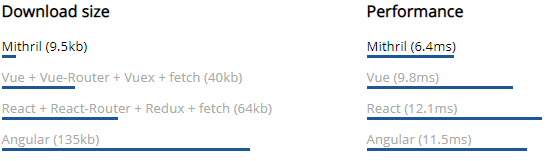
\includegraphics{fig/grundl/mithril}
	\caption{Temp Caption}
	\label{fig:mithril}
\end{figure}


\subsubsection{Installation}
\label{ssec:mithril:install}

Die installation kann auf verschiedene Wege realisiert werden.

Wenn es einen Node.js server gibt, dann kann Mithril mithilfe des Node-Package-Managers installiert werden.
Daf�r muss nur der folgende Befehl im Terminal eingegeben werden, wenn man sich im richtigen Ordner befindet.

\begin{itemize}
	\item npm install mithril
\end{itemize}

Ein anderer Weg ist �ber das Content Delivery Network (CDN). Daf�r muss der Link einmalig in Body der root HTML-Datei eingebunden werden. Im normalfall handelt es sich hier um die index.html.

\begin{lstlisting}[caption= CDN-Link f�r Mithril]
	<script src="https://unpkg.com/mithril/mithril.js"></script>
\end{lstlisting}

Auch ein sehr intressanter Weg das Framework zu nutzen, ist es lokal einzubinden. Daf�r muss eine Javascript-Datei erstellt werden, die die Distribution des Frameworks beinhaltet. Die Distribution kann mithilfe von unpk gefunden werden oder auf dem Github repository des Frameworks.

\subsubsection{Wichtige Mithril Funktionen}
\label{ssec:mithril:wichtig}

Die m-Funktion ist eine Hyperscript-Funktion die es erlaubt jedes DOM-Element zu erstellen, das HTML besitzt. Zum Beispiel kann ein div damit erstellt werden. Das dieses div aber mit Mithril erstellt wurde, ist kein echtes DOM sondern ein Virtual-DOM oder auch vnode genannt. Das vnode ist ein JavaScript Objekt was an ein echtes DOM angeh�ngt wird. Es reagiert auf ver�nderung deutlich schneller als ein echtes. Das DOM-Element an das die vnodes angeh�ngt werden ist dabei fast immer der Body. Die Schreibweise ist sehr Kompakt und kann sehr �bersichtlich gestaltet werden.

Die Funktion nimmt drei Argumente getrennt mit einem Komma an. Das erste Argument ist das HTML-Element was erstellt werden soll. Wenn dieses Feld leer bleibt, handelt es sich um ein div. Das zweite Argument sind die Attribute die es haben kann. Diese sind optional. Die Attribute werden in geschweiften Klammern geschrieben. Darin k�nnen sich styles befinden. Das letzte argument ist das Child. Das der Wert zwischen den HTML-tag. Also das was auf der Ausgabe in der Webseite angezeigt werden soll. Au�erdem kann man noch eine k�rzere schreibweise f�r die Klassen und ID Selektoren f�r CSS verwenden, indem man diese mit . f�r Klasse und \# f�r ID in das erste Argument schreibt. Im folgenden Beispiel wird dies nochmal deutlich gemacht.

\begin{lstlisting}[caption=Beispiel einer konfigurierten m().]
	m("div.klasse", \{id: "box"\}, "hello")
	//Equivalent in HTML:
	//<div id="box" class="klasse"> Hallo </div>
\end{lstlisting}

In folgendem Beispiel wird noch das zweite Argument n�her erkl�rt. Dabei werden dem button drei Attribute �bergeben. Alle Attribute m�ssen in die geschweifte Klammer und werden mit Kommas voneinander getrennt.

\begin{lstlisting}[caption={Einbinden von Klassen, Eventhandlern und Lifecycle Methoden}]
	m("button", {
		class: "my-button",
		onclick: function() {/* ... */},
		oncreate: function() {/* ... */}
	})
\end{lstlisting}


\subsubsection{Mithril Komponente}
\label{ssec:mithrilKomponente} 

Eine Komponente ist ein JavaScript Objekt und sie kann eine View-Funktion beinhalten. Au�erdem kann eine Komponente Funktionen enthalten. Lokale Variablen k�nnen in eine solche Komponente erstellt werden. Der zugriff auf diese Variablen ist �ber das Ansprechen der Komponente und die darin befindlichen variablen mit dem Punkt-Operator m�glich. Die Komponente kann auch komplett mit der Model-View-Controller Architektur erstellt werden. 
Um Daten in eine Komponente zu �bertragen muss das �ber das attrs-Objekt von Mithril erfolgen. Ein Beispiel um dieses vorgehen zu verstehen:

Um zugriff auf die Komponenten zu bekommen muss die Komponente exportiert und importiert werden, wie in folgenden Beispielen aufgezeigt wird. 

\begin{lstlisting}[caption=Zugriff auf Daten einer importierten Komponente.]
	import BeispielKomponente from "./BeispielKomponente.js"
	const beispielVariable = BeispielKomponente.beispielData;
\end{lstlisting}

\begin{lstlisting}[caption=Exportieren einer Komponente.]
	let BeispielKomponente : {
		beispielData: "Hallo",
	}
	export default BeispielKomponente;
\end{lstlisting}

\subsubsection{Mithril REST-Anfragen mit m.request}
\label{ssec:rest}

Mithril liefert eine Funktion mit der man Anfragen schicken kann. Die sogenannte m.request(). Die Funktion �hnelt sehr der JavaScript Fetch-API.
Als Response bekommt man immer ein Promise zur�ck. Egal ob die Anfrage Problemlos funktioniert hat oder nicht.

\begin{lstlisting}[caption=Promise einer REST-Anfrage mit m.request().]
	Promise {<pending>, constructor: ?, then: ?}
	constructor: ? PromiseProxy(executor)
	then: ? ()
	__proto__: Promise
	catch: ? catch()
	constructor: ? Promise()
	finally: ? finally()
	then: ? then()
	Symbol(Symbol.toStringTag): "Promise"
	__proto__: Object
	[[PromiseState]]: "fulfilled"
	[[PromiseResult]]: undefined
\end{lstlisting}

Die Anfrage braucht mindestens eine definierte HTTP-Methode und die URL von der aus die Daten angefragt oder hinterlegt werden sollen. Je nachdem was es f�r eine Methode ist muss auf weiteres geachtet werden. F�r die GET-Anfrage ist es m�glich in der URL einen Suchbegriff oder �hnliches einzuf�gen. Daf�r einfach �ber String-Verkettung mit einem + den erwarteten input weiterleiten.

\begin{lstlisting}[caption=Beispiel: Request der Methode GET mit Benutzereingabe.]
	
	let getRequestWithUserInput = {
		
		fetchExample: function (usereingabe) {
			return m.request({
				method: "GET",
				url: "URL" + usereingabe,
			})
		}	
		
	\end{lstlisting}
	
F�r weitere M�glichkeiten wie die PUT oder Post k�nnen auf der Dokumentationsseite von Mithril.js recherchiert werden.

Um nun mit den Daten der Antwort arbeiten zu k�nnen, kann wie im n�chsten Beispiel einen .then / .catch Block angewendet werden. 

\begin{lstlisting}[caption=Beispiel: m.request().then().catch().]
	
	let fetchExample = {
		response: [],
		
		fetchEx: function (input) {
			return m.request({
				method: "GET",
				url: "URL" + input,
			}).then(function (data) {
				try {
					fetchExample.response = data;
				} catch (error) {
					console.log("Error:" + error);
				}
			});
		}	
\end{lstlisting}
	
	
\subsubsection{Lebenszyklen in Mithril}

Komponenten k�nnen �ber eine oder mehrere Lebenszyklus Methode verf�gen, die an verschiedenen Punkten w�hrend der Lebensdauer eines DOM-Elements aufgerufen werden kann. Die von Mithril unterst�tzten Lebenszyklus Methoden sind: oninit, oncreate, onupdate, onbeforeremove, onremove und onbeforeupdate.
	
Die Lebenszyklen werden sp�testens dann wichtig wenn eine Fetch-Anweisung Daten von einer Schnittstelle laden soll. Die dabei unterschiedlich lange dauern kann. Dadurch ist nicht automatisch gew�hrleistet ob eine komponente zugriff auf die Daten hat, wenn diese erstellt wurde. F�r so einen Fall empfielt sich die Mehtode oninit. Dabei werden die Daten als erstes geladent und erst wenn diese Vollst�ndig da sind wird die Komponente gebaut. 
	
\subsubsection{Mithril Routen}
	
Das Routen oder Navigieren der Seiten in einer Anwendung ist ein essentieller Bestandteil jeder Webapplikation und Webseite. Diese ist in Mithril wie folgt gel�st. Mithril verwendet daf�r eine eigene Mehtode. Die methode wird m.route genannt und wie in folgendem Beispiel angewendent. Dabei wird einfach eine Komponente eingebaut die angezeigt werden soll. Das erreicht man zum Beispiel durch eine Statusvariable.

Der Aufbau sieht wie folgt aus:

\begin{lstlisting}[caption=Aufbau der m.route-Funktion.]		
		m.route(root, defaultRoute, routes)	
\end{lstlisting}	

Die Funktion verlangt 3 Parameter. Der erste ist das DOM-Elemnt an das alles angeh�ngt wird. Wie zum Beispiel das Body Element das �ber document.body erreichbar ist. Der zweite Parameter ist eine Default Route damit eine Startseite angezeigt werden kann. Der dritte Parameter ist ein Objekt mit weiteren Routen.

Ein Beispiel aus der Demo sieht wie folgt aus:

\begin{lstlisting}[caption=Aufbau der m.route-Funktion.]		

m.route(document.body, "/home", {
	"/home": {
		render: function () {
			return m(home);
		},
	},
	"/country": {
		render: function () {
			return m(country);
		},
	},
	"/vaccine": {
		render: function () {
			return m(vaccine);
		},
	},
	"/allCountries": {
		render: function () {
			return m(allCountries);
		},
	},
});
\end{lstlisting}	

Wie in dem Beispiel zu sehen, wird immer die entsprechende Komponente, die auch die View beinhaltet �bergeben. 
Um die Routen in der Navigationsleiste richtig aufzurufen baut man einen Link ein der im href die route enth�lt. 
Eine m�gliche implementierung in der Navigationsleiste k�nnte wie folgt aussehen:

\begin{lstlisting}[caption=Aufbau der m.route-Funktion.]
m(
"a[href=./index.html#!home]",
	{
	/* Mit m.route.link wird der angegebene Link in href �bergeben. */
	oncreate: m.route.link,
	},
	"HOME"
),
\end{lstlisting}

\subsubsection{Dynamische Inhalte in Mithril}

Dynamische Inhalte d.h. das ver�ndern von Inhalten, oder das abrufen von Daten zur Laufzeit ist bei Beachtung der bisher beschriebenen Punkte m�glich. Sobald eine Variable ver�ndert wird, oder eine Fetch-Anweisung getriggert wird, erzwingt man damit ein neues zeichnen der jeweiligen Komponente auf der Webseite. 

\subsubsection{Fazit}

Mithril bietet im gesamten eine breites Verzeichnis f�r die Erstellung von kleinen Webanwendungen an. Eine Komponente ist dabei �bersichtlich in drei Teile aufgeteilt. F�r �bersichtlichkeit sorgt auch die Struktur, die mit der Hyper-Script-Funktion von Mithril erreicht werden kann. Auch das auslagern von Teilkomponenten ist leicht und �bersichtlich realisierbar. Die Dokumentation ist sehr Umfangreich, allerdings ist das Framework dennoch nicht leicht zu erlernen und hebt sich durch die Struktur von anderen Frameworks ab. Es ist auch nicht weit verbreitet und es hat eine vergleichsweise kleine Gemeinschaft, dadurch k�nnen Fehler erschwerter behoben werden. 

\pagebreak
\subsection{Preact}
\label{sec:preact:intro}

\subsubsection{Installation}

Preact hat eine dist.js Datei. Diese kann man entweder �ber einen CDN-Link einbinden, oder man kann sich diese Distribution kopieren und lokal in das Projekt als eigene Bibliothek einbinden. Wir haben uns dieses mal f�r eine lokale Bibliothek entschieden. Deshalb habe ich die Distribution �ber den Github Kanal heruntergeladen und lokal in das Projekt eingebunden. Allerdings muss man darauf achten ob diese auch alle Abh�ngigkeiten abdeckt. Gegenbefalls m�sste man weitere miteinander Verkn�pfen.  

\begin{lstlisting}[caption=Import der Funktionen/ Mehtoden in Preact �ber eine Lokale Distribution]
	import { h, Component } from './PfadZurBib.js'
\end{lstlisting}

\subsubsection{Struktur}

Die Struktur von Preact ist sehr �hnlich der von React. Es ist von Vorteil wenn man sich schon mit React auskennt. Die Dokumentation in Preact ist nicht so ausf�hrlich weil man vieles aus der Dokumentation von React bekommt. Es gibt dennoch signifikante unterschiede. Ein gro�er unterschied ist das Preact kein JSX unterst�tzt und man durch eine zus�tzliche Bibliothek mit dem Namen \enquote{htm} einbinden muss. htm wandelt den JSX code in normalem HTML Code um, sodass man nur jede Variable oder Komponente mit einem \enquote{\$\{Variable\}} angeben muss. Die ganze HTML Struktur wird nun in Javascript erstellt.

In folgender Abbildung ist der Aufbau einer Funktionalen Komponente die, die HTML-Struktur zur�ck gibt. Wie man auch sehen kann ist die Naviagtions-Komponente wie oben erw�hnt eingebunden. Und darunter sieht man die gewohnte HTML-Schreibweise. 

Was hier aber erstellt wird ist kein echtes HTML-Objekt. Es handelt sich hierbei um ein Virtual-DOM. 

\begin{lstlisting}[caption= Aufbau einer HTML-Struktur mit Preact]
import { h, render } from "./libs/distPreact.js";
import htm from "./libs/distPreactHTM.js";
const html = htm.bind(h);
import { Navigation } from "./Components/navigation.js";

const Home = () => {
	return html`
	<\${Navigation} />
	<footer class="footer mt-6">
		<div class="content has-text-centered">
			<p>
				<strong>Covid Demo mit Preact.js and Bulma.io</strong> erstellt von Konstantinos Tsolakidis
			</>
		</div>
	</footer>
	`;
};
render(h(Home), document.body);

\end{lstlisting}


\subsubsection{Klassen-Komponente}

Eine Klassen Komponente erbt von der preact-Methode Component. Sie braucht au�erdem einen Konstruktor. In diesen Konstruktor werden dann die States d.h. die Statusvariablen der Klassenkompononte erstellt. Au�erdem ist man gezwungen an jede Funktion in dieser Klasse das this an jede Funktion im Konstruktor anzubinden.
Sie enth�lt au�erdem noch eine Mehthode rendern() die das HTML zur�ckgibt. Es wird in diesem Fall mit htm als HTML geschrieben und nicht wie in React in JSX. 
Mit einer Ver�nderung der States wird ein neu rendern ausgel�st. Hinzu kommt das man sich jetzt auch mit den Lebenszyklen befassen muss. Denn es gibt einige dieser Methoden, aber eine dieser Methoden ist sehr wichtig. Die Methode ComponentDidMount() wird dazu genutzt um Datenzugiff einer Fetchanweisung zu garantieren, denn diese sorgt daf�r das wenn die HTML Struktur aufgebaut wurde auch der Zugriff auf die Dateien erfolgt. 

\subsubsection{Funktionale-Komponenten}

Eine Funktionale Komponente wird mit der neuen Schreibweise von ES6 erstellt. Das hei�t es werden Pfeil Funktionen erstellt. Der gro�e Vorteil hierbei ist die kurze Schreibweise und der Entfall des this.

Um in einer Funktionales Komponente mit States zu arbeiten wird die Hauseigene Methode der Hooks von Preact angewendet. Daf�r muss die Hooks Bibliothek importiert werden. Diese beinhaltet dann zwei Methoden. Eine ist die useState() und die zweite ist die useEffect(). Die useState wird f�r die States verwendet. Dabei wird in einer Zeile der Typ des States in den Klammer des useStates() geschrieben und auf der anderen Seite ein Setter und die eigentliche Variable die den Wert beinhaltet.

Die useEffect() ist eine Lebenszyklus-Methode die genau wie die ComponentDidMount() funktioniert. Dabei werden alle Funktionen die in dieser Methode aufgerufen werden garantiert nach der Erstellung des DOM-Baums zur Verf�gung stehen.

\subsubsection{ Lebenszyklen }



Lifecycle method			When it gets called
componentWillMount			before the component gets mounted to the DOM
componentDidMount			after the component gets mounted to the DOM
componentWillUnmount		prior to removal from the DOM
componentWillReceiveProps	before new props get accepted
shouldComponentUpdate		before render(). Return false to skip render
componentWillUpdate			before render()
componentDidUpdate			after render()

\subsubsection{HTTP-REST Anfrage mit Preact}

Preact besitzt keine eigene Fetch-Methode. Es wurde die Javascript Fetch-API benutzt.

\subsubsection{ Preact States und Props }

States werden �ber den Konstruktor in einer Klassenkomponente oder in der useState() in einer Funktionalen Komponente erstellt und benutzt.
Die Props sind dazu da um Daten in Child-Komponenten zu versenden. Daf�r werden die daten mit einer Beliebigen Variable in den HTML-Code der Komponente geschrieben.
In folgendem Beispiel bekommt die Komponente Modal einen Prop �bergeben. Dieser Prop kann dann in der Komponente Modal �ber prop.data aufgerufen und benutzt werden.

\begin{lstlisting}[caption=Preact Props einer Komponente �bergeben.]
	
    <${Modal} data=${currentCountry} active=${active} />
	
\end{lstlisting}

\subsubsection{ Preact Routing}

F�r das Routing wird eine Bibliothek mit dem namen Preact-Router genutzt und noch eine mit dem Namen history. 

Wie im folgenden Beispiel zu sehen werden in der Router Komponente die Pfade gesetzt.
Damit diese auch besser gefunden werden und auch die zur�ck taste im Browser verwendet werden kann, wird der gebrauch von createHistory() verwendet.


\begin{lstlisting}[caption=Preact Router mit history.]
	
<${Router} history=${createHashHistory()} >
	<${HomePage} path="/" />
	<${Dashboard} path="/dashboard"/>
	<${Vaccine} path="/vaccine"/>
	<${Country} path="/country"/>
</$>

\end{lstlisting}

In folgendem Codebeispiel sieht man die Einbindung einer Route in die Navigationleiste. Hierf�r wird ein Link-Tag benutzt und mit der Route und einem onClick-Handler versehen.

\begin{lstlisting}[caption=Route in einem Link eingebunden.]
<a class="navbar-item" href="/country" onClick=${()=> setActive("")}>
\end{lstlisting}

\subsubsection{Dynamische Inhalte in Preact}

Dynamische Inhalte sind in Preact einfach zu gestalten. Daf�r muss mit den States gearbeitet werden. Diese f�hren einen neues rendern aus. Die Ver�nderung der States werden sofort auf der Seite angezeigt.

\subsubsection{Fazit}

Preact ist eine abgespeckte Version von React. Dabei kann es und muss es teilweise erweitert werden. Preact braucht die Bibliothek \enquote{HTM}. Auch die Benutzung von Bibliotheken die f�r React gedacht sind, sind teilweise kompatibel mit Preact. Es ist deutlich kleiner (3KB) als React (45KB) und auch von der Performance schneller, dies macht es f�r mobile Ger�te sehr Interessant. Dabei ist die gr��te Einsparungen, dass weglassen von einem Hauseigenen synthetischen Event System. Preact verl�sst sich auf den Haus eigenen Eventlistener der vom Browser zur Verf�gung gestellt wird. Allerdings ist das nur ein Teil der Funktionen von React darunter fehlen noch PropTyps und children.  Ein weiterer Punkt der auch zu beachten ist, ist das Preact eine deutlich kleinere aktive Gemeinschaft hat. Das macht es schwieriger bei Problemen oder Fehlern den Grund aufzufinden. Die Dokumentation ist recht klein, da auch manches in der Dokumentation von React nachgeschlagen werden kann. Die Struktur ist sehr sauber und das arbeiten mit Funktionalen Komponenten und Hooks spart sehr viele Zeilen Code und erleichtert dabei auch mit dem Verst�ndnis. Auch ist durch den Einsatz von \enquote{HTM} eine nahezu identische Erstellung einer \enquote{normalen}-HTML Struktur m�glich. Dadurch spart man sich viel Zeit beim erlernen des Frameworks. 

\pagebreak
\section{Untersuchung von CSS-Frameworks}
\subsection{Purecss}
\label{sec:demomithril:intro}

Purecss ist im gesamten ein 3.7 KB Gro�es Framework. Es ist Modular aufgebaut. Darunter befinden sich insgesamt 6 einzeln benutzbare Module. Diese sind unabh�ngig voneinander Installierbar und k�nnen somit deutlich weniger Speicherplatz einnehmen. Da die Module sehr klein sind, haben diese deswegen auch keine gro�e Auswahl. Aber f�r kleine Projekte reichen die Module aus. In der Abbildung 2 ist die Modulare Aufteilung mit ungef�hrer Speichergr��e abgebildet.
Unter folgendem Link: https://purecss.io/customize/ stehen die Links f�r jedes einzelne Modul.

\begin{figure}
	\centering
	
\includegraphics[width=0.7\linewidth]{../Purecss_Module}
	\caption{}
	\label{fig:purecssmodule}
\end{figure}

\subsubsection{Installation / Einbindung in das Projekt}

Man kann das Framework �ber CDN (Content Delivery Network) einbinden. Daf�r muss lediglich der folgende Link in den Head der HTML Datei eingef�gt werden.

\begin{lstlisting}[caption=Einbinden von purecss.io]
	
<link rel="stylesheet" href="https://unpkg.com/purecss@2.0.5/build/pure-min.css" integrity="sha384-G9DpmGxRIF6tpgbrkZVcZDeIomEU22LgTguPAI739bbKytjPE/kHTK5YxjJAAEXC" crossorigin="anonymous">

\end{lstlisting}

\subsubsection{Pure Grid Layout}

Das Gridlayout von purecss ist einfach aufgebaut und l�sst sich komplett individualisieren. Die Grids lassen sich in zwei Gruppen aufteilen. Dabei hat es die Einteilung in grob und fein. Dabei kann beim groben layout eine Einteilung von 5 Spalten erreicht werden. Bei der feinen sogar 24. Um ein solches Layout zu realisieren, muss als erstes ein Div erstellt werden, dass als Container dient. Dieses bekommt die Klasse pure-g. In diesen kommen dann die einzelnen Elemente mit der Klasse pure-u-*. Dabei steht das Sternchen f�r die jeweilige Breite, die erreicht werden soll. Diese kann zum Beispiel von der ganzen Breite bis hin zu einem vierundzwanzigstel klein sein. Des weiteren lassen sich auch Bilder in die einzelnen Spalten integrieren. Daf�r muss ein img-Tag in das div mit der Klasse pure-img integriert werden. Dabei wird das Bild responsive und l�sst sich dynamisch skalieren. 

In n�chsten Beispiel wird gezeigt, wie die sich der Klassenname zusammenstellt, wenn man diese wie in css mit der Media Query anpassen m�chte. Dabei wird in jeder Klasse der entsprechende Key eingebaut. Somit schreibt man f�r kleine Endger�te unter 568px ein sm f�r small und f�r Ger�te gr��er 1280px ein xl f�r extra Large. 

Das Gridlayout funktioniert nur bei dem div-Element.

\begin{lstlisting}[caption= Aufteilung der @media screen gr��en in purecss.io]
	
	Key			CSS Media Query										 Applies	      Classname
	None		None													  Always	       .pure-u-*
	sm		@media screen and (min-width: 35.5em)	   ? 568px		  .pure-u-sm-*
	md		@media screen and (min-width: 48em)			? 768px		   .pure-u-md-*
	lg		  @media screen and (min-width: 64em)		  ? 1024px		.pure-u-lg-*
	xl		  @media screen and (min-width: 80em)	   	  ? 1280px		.pure-u-xl-*	
	
\end{lstlisting}

In folgendem Codebeispiel wird veranschaulicht wie das Gridlayout von purecss in Mithril bei einem div eingebunden wird.

Die Gr��e des Endger�tes bestimmt nun wie viel Platz das Div auf dem Bildschirm bekommt.
Auf einem mobilen Endger�t wie dem Smartphone w�rde dieses Div 100 Prozent des Bildschirm einnehmen.
Bei einem Tablet w�ren das, dann nur noch 50 Prozent und bei einem Desktop PC mit einem Monitor Gr��er als 1024px nur 25 Prozent der Bildschirmbreite.

\begin{lstlisting}[caption=Beispiel: Responsive Grid implementieren in MithrilJs.]

m("div.pure-u-1 pure-u-md-1-2 pure-u-lg-1-4",{attrs},child)	
m("div.pure-u-1 pure-u-md-1-2 pure-u-lg-1-4",{attrs},child)
m("div.pure-u-1 pure-u-md-1-2 pure-u-lg-1-4",{attrs},child)	
m("div.pure-u-1 pure-u-md-1-2 pure-u-lg-1-4",{attrs},child)	
\end{lstlisting}


 \subsubsection{Pure Buttons}
 
	Das Button Modul ist ein sehr kleines und praktisches Modul. Es beinhaltet keine sehr gro�e Auswahl an verschiedenen Kn�pfen. Aber die Styles, die es anbietet sind durchaus brauchbar und k�nnen sich trotzdem sehen lassen. Neben den Standard Kn�pfen in Grau gibt es auch welche f�r einen aktiven und inaktiven Knopf. Au�erdem bietet Pure auch den Primary Button der oft in Blogs oder Shops seinen Platz findet. Zuz�glich zur Primary Farbe gibt es 4 weitere. Gr�n, Rot, Orange und Hellblau die alle einen sehr aussagekr�ftigen aber nicht st�renden Farbton haben. Dabei steht Gr�n f�r einen Erfolgreichen Knopfdruck, Rot f�r einen Fehler, Orange f�r eine Warnung und Hellblau f�r den Secondary Knopf. Als letzte Eigenschaft kann die Gr��e ver�ndert werden.
	Die gr��en sind dabei von der Schriftgr��e abh�ngig. Die kleinste Gr��e ist .button-xsmall und das entspricht der Font-Gr��e von 70\% und der Gr��te Knopf ist der .button-xlarge und entspricht der Font-Gr��e 125\%.
 
  \subsubsection{ Pure Forms }
 
Es gibt 5 verschiedene  Form-Felder die direkt �rbernommen werden k�nnen. Dabei gibt es die Standard Form f�r den Login mit Email, Password, einem check Feld und einem Button. Diese ist Horizontal angeordnet und f�r jedes Beispiel ist der Aufbaus in einer HTML-Struktur abgebildet. Die Felder lassen sich sogar in einem Gridlayout verbinden sodass man eine Form bekommt die f�r Kundendaten geeignet ist. 

Die Demo hat f�r das Suchfeld die Form mit den abgerundeten Ecken bekommen. 
\begin{lstlisting}[caption=Verwendete Pure Form in der Demo]
<form class="pure-form">
	<input type="text" class="pure-input-rounded" />
	<button type="submit" class="pure-button">Search</button>
</form>
\end{lstlisting}

\subsubsection{ Fazit }

Pure ist ein sehr kleinen Framework was das minimalste an Styles mit sich bringt. F�r kleinere Webanwendungen die keine gro�en extras wie Karten oder Modals brauchen, eignet es sich gut. Es ist sehr klein und kann durch seine Modularit�t noch kleiner werden, da auch nur die erw�nschten Module installiert werden k�nnen. Die Dokumentation ist sehr Gut und die Handhabung sehr einfach. 

  \pagebreak
 \subsection { Bulma } 
 
 Bulma ist ein open source Framework das ohne JavaScirpt geliefert wird. Des weiteren ist es Modular. Das bedeutet, dass man auch einzelne Module installieren/ downloaden kann. Deshalb ist es f�r alle Projektgr��en geeignet. Derzeit ist es in sechs Module unterteilt. Darunter befinden sich die Module Columns, Elements, Components, Forms, Layout und Helpers. 
 
 
 \subsubsection{ Installation }
 
 Die Installation erfolgt entweder �ber CDN oder �ber npm (Node Package Manager). 
 Unter folgendem Link: https://bulma.io/documentation/overview/start/ sind die Schritte f�r die Installation beschrieben. Mit dem Link: https://bulma.io/documentation/overview/modular/ sind die Schritte f�r die Modulare Installation des Frameworks beschrieben.
 
 
 \subsubsection{ Modul Elemente}
 
 Das Elements Modul ist eines der essentiellen. Darin befinden sich 12 Elemente wie Block, Box, Button, Content, Delete, Icon, Image, Notification, Progress bars, Table, Tag und Title. In der Demo wurde von Block, Button, Content und Title gebrauch gemacht. Das Element Block wird daf�r verwendet einen Abstand zwischen anderen Elementen zu schaffen. Das Element Title wird zusammen mit Subtitle verwendet. Beide haben 6 verschiedene Gr��en. Wenn Title und Subtitle direkt untereinander benutzt werden r�cken diese etwas n�her zusammen. Das Content Element wird nur f�r Text verwendet. Darin d�rfen sich nur html-Elemente wie paragraphs, lists, headings, quotes und tables befinden. 
 
 \subsubsection{ Modul Layout}
 
 Im Modul Layout befinden sich Styling Komponenten f�r die Formatierung von Texten und Abschnitten. F�r die Demo wurde die Klasse Container und Section verwendet. Um das Styling in das Projekt zu bekommen muss lediglich der Name Container an ein div-tag als Klasse �bergeben werden. Bei der Klasse Section braucht es ein section.tag.
 
 \begin{lstlisting}[caption=Beispiel: Klassen Anwendungsbeispiel in Bulma]
 	
 	<div class="container">	
 	<section class="section">
 	<h1 class="title">Section</h1>
 	<h2 class="subtitle">
 	A simple container to divide your page into <strong>sections</strong>, like the one you're currently reading.
 	</h2>
 	</section>
 	</div>
 	
 \end{lstlisting}
 
 Es ist auch m�glich weitere Ver�nderungen vorzunehmen. Zum Beispiel wie breit der Container sein soll mit .is-widescreen oder .is-fullhd. Der Container wird genutzt um den Inhalt mittig zu fixieren. Somit ist er immer mit und hat einen default Mindestabstand von 32px zur Au�enkante des Bildschirms. 
 
 
 
 \subsubsection{ Modul Form}
 
 Das Form Modul sorgt f�r eine Klare Struktur und �bersichtlichkeit des Steuerelements Form. In diesem Modul werden folgende HTML-Elemente gestyled:
 
 label, input, textarea, select, checkbox, radio, button und help.
 
 Im Allgemeinen bietet Bulma f�r die g�ngigsten Form Anwendungsf�lle solide L�sungen. Diese sind Modern und Schlicht gehalten. K�nnen aber auch mit Icons Individualisiert werden. Dabei reichen die vorgefertigten L�sungen von einer normalen Anmeldung mit Email bis zu Feldern die mit W�hrungen und Online-shops zu tun haben.
 
 \subsubsection{Navigation, Karte und Modal mit dem Modul Komponente}
 
 Das Modul Komponente besteht aus 10 Elementen. Darunter befinden sich die Komponenten:
 Breadcrumb, Card, Dropdown, Menu, Message, Modal, Navbar, Pagination und Panel. 
 Die Elemente sind in grob in zwei Gruppen aufzuteilen. Die erste Gruppe ist die, der Navigation. Das hei�t f�r die Darstellung von Hierarchien und das Navigieren zwischen verschiedenen Seiten. Die zewite Gruppe ist f�r Effekte und �bersicht geeignet. Die Auslagerung von Informationen wie in einem dropdown Men� oder einem Modal ist hier m�glich. Auch eine sch�ne und �bersichtliche Darstellung von zusammengeh�renden Inhalten kann mit einer Karte realisiert werden. F�r die Demo wurde die Navigation, die Karte und das Modal verwendet. Die Navigation ist schon f�r kleine und gro�e Ger�te optimiert. Wenn ein Smartphone verwendet wird wechselt die Navigation in ein Burger-Men�. Bei einem Desktop mit mehr als 1200 Pixel breite wird die Navigation Horizontal oder Vertikal mit allen einzelnen Elementen angezeigt. Das �ffnen und schlie�en der dropdown Eigenschaften wie beim Burger-Men� wird �ber den Klassennamen is-active ver�ndert. Das kann mit Javascript und dem dazugeh�rigen Framework in unterschiedlichen Variationen gel�st werden. Das gleiche gilt auch f�r das Modal, dass auch durch den Klassennamen is-active gesteuert wird.
 
 
 \subsubsection{ Individualisierung mit dem Modul Helpers }
 
 Jede Komponente kann noch Individualisiert werden. Und das ohne eine Zeile Code in einem CSS Dokument zu schreiben. Punkte wie das Margin zu anderen DOM-Elementen oder auch die Textfarbe lassen sich einfach mit dem Klassennamen m* f�r margin und p* f�r padding und die dazugeh�rige Seite wie t f�r Top erstellen. Wenn jetzt der Abstand von oben vergr��ert werden soll muss lediglich ein mt-(0-6) eingegeben werden. Die values sind von 0 - 6 und mit einem abstand von 0 , 0.25 rem bis 3 rem gestuft. REM ist relativ zur html fontgr��e dagegen ist em abh�ngig von direkt umligenden Elternknoten.
 
 \subsubsection{Fazit}
 
 Bulma ist ein modernes und Modulares Framework. Es ist responsive und f�r mobile first designed. Die Dokumentation ist sehr Umfangreich und leicht verst�ndlich. Die Anwendung ist sehr einfach. Jede Komponente hat ein Beispielcode der die HTML-Struktur aufzeigt. Durch die 39 .sass Dateien lassen sich auch nur die Module einbinden die auch gebraucht werden. Deshalb ist die gr��e des Frameworks individuell einstellbar und anpassbar nach den Bed�rfnissen.
 
 \pagebreak
 \section{Untersuchung von ArangoDB}
 
 in bearbeitung...
 
 \pagebreak
 \section{Untersuchung von Foxx-microservice Framework}
  
 in bearbeitung...

%\FloatBarrier
\section{Hauptteil}
\label{sec:haupt:intro}

%\begin{table}[h!]
%	\centering
%	\begin{tabular}{p{0.3\linewidth}|p{0.7\linewidth}}
%		\toprule
%		\textbf{Parameter} & \textbf{Beschreibung} \\ 
%		\midrule
%		$a_1 = 0.05$ & Zuwachsrate der Beutetiere durch Geburten \\
%		\midrule
%		$b_1 = 0.02$ & nat�rliche Todesrate der Beutetiere \\
%		\midrule
%		$c_1 = 0.0006$ & Fressrate der R�uber \\
%		\midrule
%		$a_2 = 0.0002$ & Zuwachsrate der R�uber durch Geburten \\
%		\midrule
%		$b_2 = 0.1$ & nat�rliche Todesrate der R�uber \\
%%		\midrule
%%		$x_{10} = 2500$ & Anfangszahl Beutetiere \\
%%		\midrule
%%		$x_{20} = 10$ & Anfangszahl R�uber \\
%		\bottomrule
%	\end{tabular}
%	\caption{Parameter der Lotka-Volterra-Modelle}
%	\label{tab:haupt:param}
%\end{table}

\subsection{Model \RN{1}: Unbegrenztes Populations-Modell}
\label{sec:haupt:model1}

\subsubsection{Realisierung in MATLAB}
\label{sec:haupt:matlab1}
%Im Folgendem wird erl�utert, wie das Modell 1 der Lotka-Volterra-Gleichungen in MATLAB umgesetzt werden kann. Hierzu erfolgt, in einem ersten Schritt, die Diskretisierung bzw. Ann�herung der Zustandsdifferentialgleichungen aus \autoref{sec:grundl:gl}. Diese kann, basierend auf \cite[S. 262, 296, 532 f.]{lit:Koch2015}, wie folgt definiert werden:

\begin{align}
	\frac{dx}{dt} = \dot{x} &\approx \frac{x_k - x_{k - 1}}{h} \nonumber \\
	x_k &= x_{k - 1} + h \cdotp \dot{x} 
	\label{eqn:haupt:diskret}
\end{align}

\autoref{eqn:haupt:diskret} beschreibt die Linearisierung einer Funktion $x(t)$. Dadurch ist eine Ann�herung der Zustandsgr��en $x_1$ und $x_2$ m�glich. Die momentane �nderung pro Iterationsschritt ist durch $\dot{x}$ gegeben und l�sst sich anhand von \autoref{eqn:grundl:x1} und \autoref{eqn:grundl:x2} berechnen. Die Gr��e $h$ beschreibt die Schrittweite zwischen den Ann�herungen. Diese Ann�herung basiert auf dem Polygonzugverfahren von Euler (vgl. \cite[S. 534]{lit:Koch2015}). Die Beschreibung der kontinuierlichen Gleichungen in diskreter Form erm�glicht und vereinfacht die Implementierung.
\\
\\
Der gesamte MATLAB Code ist hierbei unter \autoref{lst:matlab1:code} gegeben. In einem ersten Schritt m�ssen die Parameter $a_1, b_1, c_1, a_2$ und $b_2$ mit den entsprechenden Anfangswerten deklariert und initialisiert werden. Au�erdem wird eine Maximaldauer $tmax = 50$ Wochen und der entsprechende Zeitschritt $dt = \frac{1}{7}$, der einer �nderung von einem Tag entspricht, festgelegt. Diese k�nnen dazu verwendet werden, um den Zeitvektor $t = \{0, 0+dt, 0+2 \cdot dt, \ldots, tmax-dt, tmax\}$ zu erstellen.

\begin{lstlisting}[style=Matlab-editor,caption={Deklarieren und initialisieren von Parametern},captionpos=b,label=lst:matlab1:param,language=Matlab,basicstyle=\mlttfamily,numbers=none,frame=single,escapeinside={*@}{@*}]
%% Randbedingungen / Parameter [pro Woche]

% Beute / Hasen
a1 = 0.05; % Geburtenrate: Verdopplung der Population in 20 Wochen
b1 = 0.02; % Sterberate: 2% der Hasen sterben an nat�rlichen Ursachen
c1 = 0.0006; % Fressrate der F�chse

% R�uber / F�chse
a2 = 0.0002; % Geburtenrate/Beutewahrscheinlichkeit der F�chse
b2 = 0.1; % Sterberate: F�chse verlieren pro Woche 10% Biomasse

% Anfangsbedingungen
dt = 1/7; % Zeitschritt
tmax = 51*10; % Dauer in Wochen
t = 0:dt:tmax; % Zeitvektor
\end{lstlisting}

Um die bereits genannten Anfangszust�nde abzubilden, werden zwei \emph{for}-Schleifen durchlaufen, in denen $x1$ und $x2$ die entsprechenden Anfangswerte annehmen. Hierbei werden somit sechs verschiedene Anfangszust�nde abgebildet. F�r jede Kombination dieser Anfangswerte wird, f�r jeden Zeitschritt, der entsprechende Wert f�r $x1$ und $x2$ bestimmt. Im ersten Zeitschritt werden hier die Zustandsvariablen mit den entsprechenden Anfangswerten initialisiert. \\In jedem weiteren Zeitschritt wird die �nderung der Beutepopulation $dx1$ sowie R�uberpopulation $dx2$ berechnet. 
\\
\\
Diese werden mit der Schrittweite $h$ multipliziert und auf den $(i - 1)$-ten Wert der Populationen $x1$ und $x2$ addiert, um so den $i$-ten Wert der Zustandsvariablen zu bestimmen. Nach dem Durchlaufen aller Zeitschritte, kann der Verlauf der Populationen grafisch dargestellt werden.
\\
\\
Nach dem Durchlaufen aller Zeitschritte sind alle Werte f�r die Zustandsvariablen berechnet. Diese werden verwendet, um die Verl�ufe der Populationen sowie die dazugeh�rige Phasenkurve darzustellen. Die einzelnen Phasenkurven werden hierbei in einen Plot eingetragen. Dies geschieht durch die Verwendung des Befehls \emph{hold(ax,'on')} bzw. \emph{hold(ax,'off')}.

\begin{lstlisting}[style=Matlab-editor,caption={Berechnen der Verl�ufe und Phasenkurven der Populationen},captionpos=b,label=lst:matlab1:calc,language=Matlab,basicstyle=\mlttfamily,numbers=none,frame=single,escapeinside={*@}{@*}]
% Eigene Axis f�r Phasenkurven
ax = gca;

%% Berechnung
for x20 = [25 10]

for x10 = [2500 1400 650]

	% mit Anfangswerten initialisieren
	x1(1) = x10;
	x2(1) = x20;
	
	for i = 2:length(t)
	
	% �nderung der Beutepopulation
	dx1 = a1*x1(i - 1) - b1*x1(i - 1) - c1*x2(i - 1)*x1(i - 1);
	x1(i) = x1(i - 1) + dt*dx1;
	
	% �nderung der R�uberpopulation
	dx2 = a2*x2(i - 1)*x1(i) - b2*x2(i - 1);
	x2(i) = x2(i - 1) + dt*dx2;
	
	end
	
	figure
	plot(t,x1,t,x2)
	xlabel('Zeit in Wochen','Fontweight','bold')
	ylabel('Population in Stk.','Fontweight','bold')
	legend('Anzahl Beute','Anzahl R�uber')
	set(gca,'Fontweight','bold')
	
	hold(ax,'on')
	plot(ax,x1,x2)
	hold(ax,'off')

end

end

xlabel(ax,'Anzahl Hasen in Stk.','Fontweight','bold')
ylabel(ax,'Anzahl F�chse in Stk.','Fontweight','bold')
title(ax,'Phasenkurve x_2 = f(x_1)')
set(ax,'Fontweight','bold')
\end{lstlisting}

Eine Alternative M�glichkeit, die Phasenkurven zu bestimmen, ist am Ende von \autoref{lst:matlab1:ode} gegeben. Hierzu werden \autoref{eqn:grundl:x1} und \autoref{eqn:grundl:x2} innerhalb einer anonymen Funktion gespeichert, die durch \enquote{@} deklariert wird. Dieser werden die Parameter $t$ und $x$ �bergeben, die entsprechend den Zeitvektor und den Vektor von Zustandsvariablen darstellen. Die Differentialgleichungen, die in dem Function Handle $f$ gespeichert sind, werden numerisch durch den \enquote{ode45}-Solver gel�st bzw. approximiert. Dieser basiert auf dem Runge-Kutta Einschrittverfahren \cite{lit:ode45}. Hierbei wird ein Zeitvektor und bestimmte Anfangswerte an den Solver als Parameter �bergeben. Die Anfangszust�nde werden hierbei mit verschiedenen Faktoren von 0.5 bis 2 multipliziert, um verschiedene Trajektorien abzubilden. Die L�sungswerte in $xs$ enthalten die angen�herten Werte der Zustandsvariablen.

\begin{lstlisting}[style=Matlab-editor,caption={Bestimmung der Phasenkurven durch den ode45-Solver},captionpos=b,label=lst:matlab1:ode,language=Matlab,basicstyle=\mlttfamily,numbers=none,frame=single,escapeinside={*@}{@*}]
figure
hold on
% Zustandsdifferentialgleichungen in anonymer Funktion speichern
f = @(t,x) [x(1)*(a1 - b1 - c1*x(2)); x(2)*(a2*x(1) - b2)];

%Phasenkurven f�r verschiedene Anfangsbedingungen bestimmen
for x20 = [25 10]

for x10 = [2500 1400 650]

	% Verlauf mit ode45 solver berechnen
	[~, xs] = ode45(f,t, [x10, x20]);
	% Phasenkurve plotten
	plot(xs(:,1), xs(:,2))

end

end

xlabel('Anzahl Hasen in Stk.','Fontweight','bold')
ylabel('Anzahl F�chse in Stk.','Fontweight','bold')
title('Phasenkurve x_2 = f(x_1)')
set(gca,'Fontweight','bold')
hold off
\end{lstlisting}

\FloatBarrier

\autoref{img:haupt:mod1_2500_25} bis \autoref{img:haupt:mod1_650_25} zeigen den Verlauf der R�uber- und Beutepopulation f�r $x_{20} = 25$. Hierbei werden f�r $x_{10} = \{2500, 1400, 650\}$ gew�hlt. Es ist zu beobachten, dass die Beutetiere, da sie die einzige Nahrungsquelle der R�uber sind, durch diese aufgezehrt werden.
\\
\\
Aufgrund dessen verringert sich die Beutepopulation rapide. Dieser Verlauf h�lt an, bis die Beutepopulation nicht mehr als Nahrungsquelle f�r die R�uber ausreicht. Dies hat zur Folge, dass sich die Anzahl der R�uber verringert. Durch eine verminderte R�uberpopulation ist es den Beutetieren wieder m�glich, sich zu vermehren. Dieses Wachstum h�lt an, bis die erh�hte Beutepopulation erneut ausreichend f�r die R�uber ist, um sich verst�rkt zu vermehren. Das Verhalten der beiden Populationen wird periodisch wiederholt.
\\
\\
Bei Betrachten der Verl�ufe, f�r die genannten Anfangswerte, hat es den Anschein, dass gr��ere Werte f�r $x_{10}$ und $x_{20}$ in einer h�heren Amplitude und l�ngeren Periode resultieren. F�r $x_{10} = 2500$ und $x_{20} = 25$ ergibt sich, aus \autoref{img:haupt:mod1_2500_25}, eine ungef�hre Periode von ca. 210 Wochen. Dies entspricht einem Zeitraum von ca. vier Jahren. Die Beutetiere erreichen hierbei eine maximale Anzahl von ca. $2500$ wohingegen die R�uber $x_2$ eine maximale Anzahl von ca. $500$ Tieren erreichen. Die Schwankungen der beiden Populationen bewegen sich hierbei, n�herungsweise, zwischen diesen Maximalzahlen.
\\
\\ 
Im Gegensatz dazu bewirken kleinere Anfangswerte $x_{10}$, bei festem $x_{20}$, scheinbar eine geringere Amplitude und Periode. In \autoref{img:haupt:mod1_650_25} ist zu erkennen, dass die Schwankungen der Populationen, f�r $x_{10} = 650$ und $x_{20} = 25$, geringer sind, als f�r $x_{10} = 2500$ und $x_{20} = 25$. Die Anzahl an Beutetieren schwankt hierbei zwischen ca. 300 und 700. Die R�uber schwanken zwischen ca. 25 und 100. Die Periode betr�gt hierbei ca. 150 Wochen. Dies entspricht ca. 3 Jahren.
\\
\\
In \autoref{img:haupt:mod1_2500_10} bis \autoref{img:haupt:mod1_650_10} sind die Verl�ufe der R�uber- und Beutepopulationen f�r $x_{20} = 10$ und $x_{10} = \{2500, 1400, 650\}$ dargestellt. Hierbei sind, f�r die Amplitude und Periodizit�t, �hnliche Aussagen wie f�r \autoref{img:haupt:mod1_2500_25} bis \autoref{img:haupt:mod1_650_25} zu treffen.
\\
\\
Es liegt die Vermutung nahe, dass geringere Anfangswerte f�r $x_1$ und $x_2$ in einer geringeren Amplitude der jeweiligen Population resultiert. Wie die Ergebnisse f�r $x_{10} = 650$ in \autoref{img:haupt:mod1_650_25} bzw. \autoref{img:haupt:mod1_650_10} zeigen, ist dies nicht immer der Fall. Es ist anzumerken, dass die Populationen, f�r beispielsweise $x_{10} = 650$ und $x_{20} = 10$, h�here Schwankungen aufweisen, als f�r $x_{10} = 650$ und $x_{20} = 25$.
\\
\\
Dieses Verhalten ist mit Hilfe der Phasenkurven zu erkl�ren. Diese sind, in \autoref{img:haupt:mod1_phasen}, f�r die Anfangswerte $x_{10} = \{2500, 1400, 650\}$ und $x_{20} = \{25, 10\}$ beispielhaft dargestellt. Hierbei sind in \autoref{img:haupt:mod1_phase} die Verl�ufe der jeweiligen Populationen in der Zustandsebene, auf Basis der mathematischen Beschreibung $x_2 = f(x_1)$, aufgetragen. In \autoref{img:haupt:mod1_phase_ode} sind die, durch den \enquote{ode45}-Solver bestimmten, Phasenkurven dargestellt. Hierbei resultieren die Ungenauigkeiten der Kurven in \autoref{img:haupt:mod1_phase_ode} aus den Ann�herungen, die der \enquote{ode45}-Solver verwendet, um die Zustandsdifferentialgleichungen zu approximieren. Aus den daraus resultierenden Fehlern resultiert eine Abweichung der Phasenkurven, die sich mit der Zeit erh�ht. Die auf dem Polygonzugverfahren von Euler basierende Implementierung in \autoref{lst:matlab1:calc} weist hierbei eine geringere Abweichung �ber der Zeit, als der auf dem Runge-Kutta Verfahren basierende \enquote{ode45}-Solver auf.
\\
\\
Durch den Anfangszustand, der durch $x_{10}$ und $x_{20}$ gegeben ist, verl�uft exakt eine dieser Trajektorien. Diese Trajektorie gibt den Verlauf der Populationen an, der sich, da es sich um geschlossene Kurven handelt, periodisch wiederholt. \\Durch den Umfang der Trajektorien ist die Amplitude des periodischen Verlaufs bzw. die Schwankungen der Populationen zu erkennen. Hierbei ist zu beobachten, dass eine Verringerung der Zustandsvariablen nicht unbedingt in einer geringeren Amplitude resultiert. Es ist ebenso m�glich, dass eine Verringerung der Anfangszust�nde, je nach Lage der Trajektorie, zu einer h�heren Amplitude f�hrt.

\FloatBarrier

\begin{figure}
	\centering
	\begin{subfigure}[h]{0.49\linewidth}
		\centering
		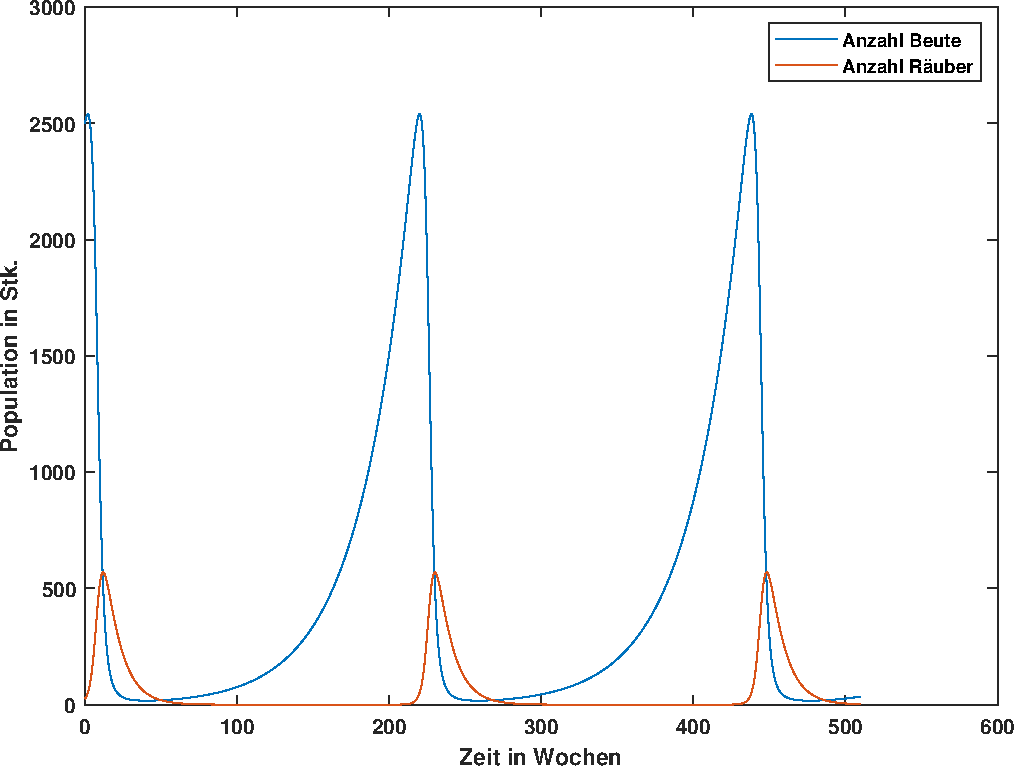
\includegraphics[width=\linewidth,height=0.8\linewidth]{fig/model/Modell1_2500_25}
		\caption{Modell \RN{1} f�r $x_{10} = 2500$ und $x_{20} = 25$}
		\label{img:haupt:mod1_2500_25}
	\end{subfigure}
	\hfill
	\begin{subfigure}[h]{0.49\linewidth}
		\centering
		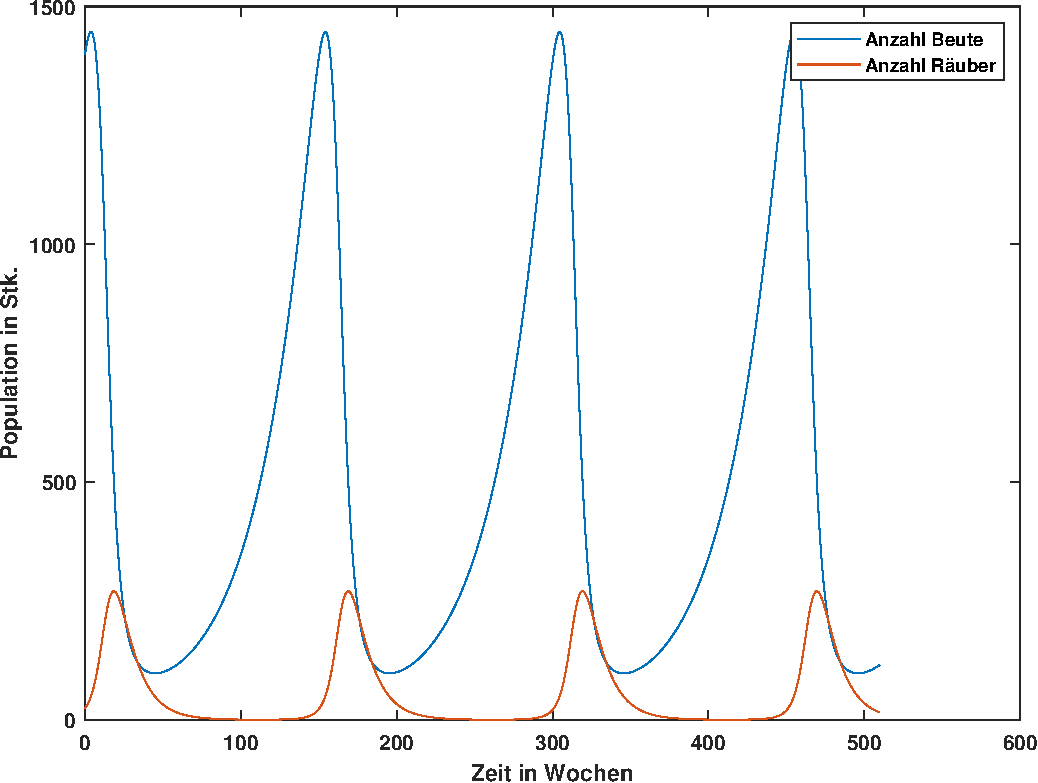
\includegraphics[width=\linewidth,height=0.8\linewidth]{fig/model/Modell1_1400_25}
		\caption{Modell \RN{1} f�r $x_{10} = 1400$ und $x_{20} = 25$}
		\label{img:haupt:mod1_1400_25}
	\end{subfigure}
	\vfill
	\begin{subfigure}[h]{0.49\linewidth}
		\centering
		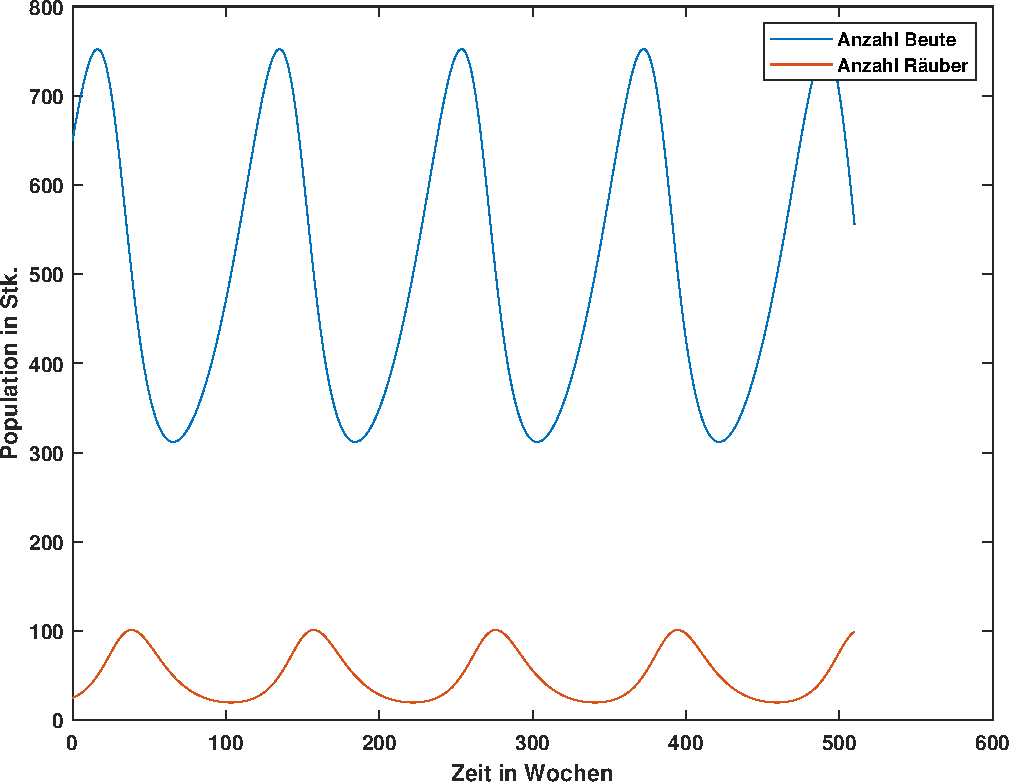
\includegraphics[width=\linewidth,height=0.8\linewidth]{fig/model/Modell1_650_25}
		\caption{Modell 1 f�r $x_{10} = 650$ und $x_{20} = 25$}
		\label{img:haupt:mod1_650_25}
	\end{subfigure}
	\caption{Modell \RN{1} f�r $x_{20} = 25$ und $x_{10} = \{2500, 1400, 650\}$}
	\label{img:haupt:mod1_x10_25}
\end{figure}

\begin{figure}
	\centering
	\begin{subfigure}[h]{0.49\linewidth}
		\centering
		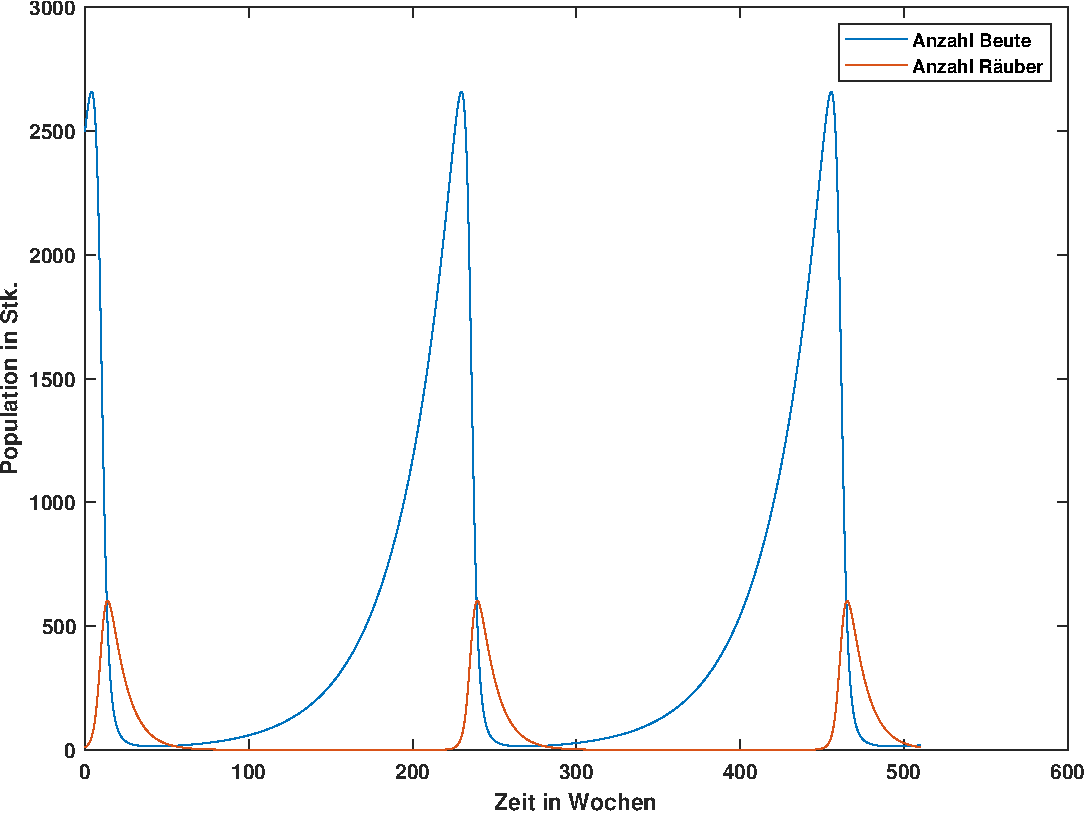
\includegraphics[width=\linewidth,height=0.8\linewidth]{fig/model/Modell1_2500_10}
		\caption{Modell \RN{1} f�r $x_{10} = 2500$ und $x_{20} = 10$}
		\label{img:haupt:mod1_2500_10}
	\end{subfigure}
	\hfill
	\begin{subfigure}[h]{0.49\linewidth}
		\centering
		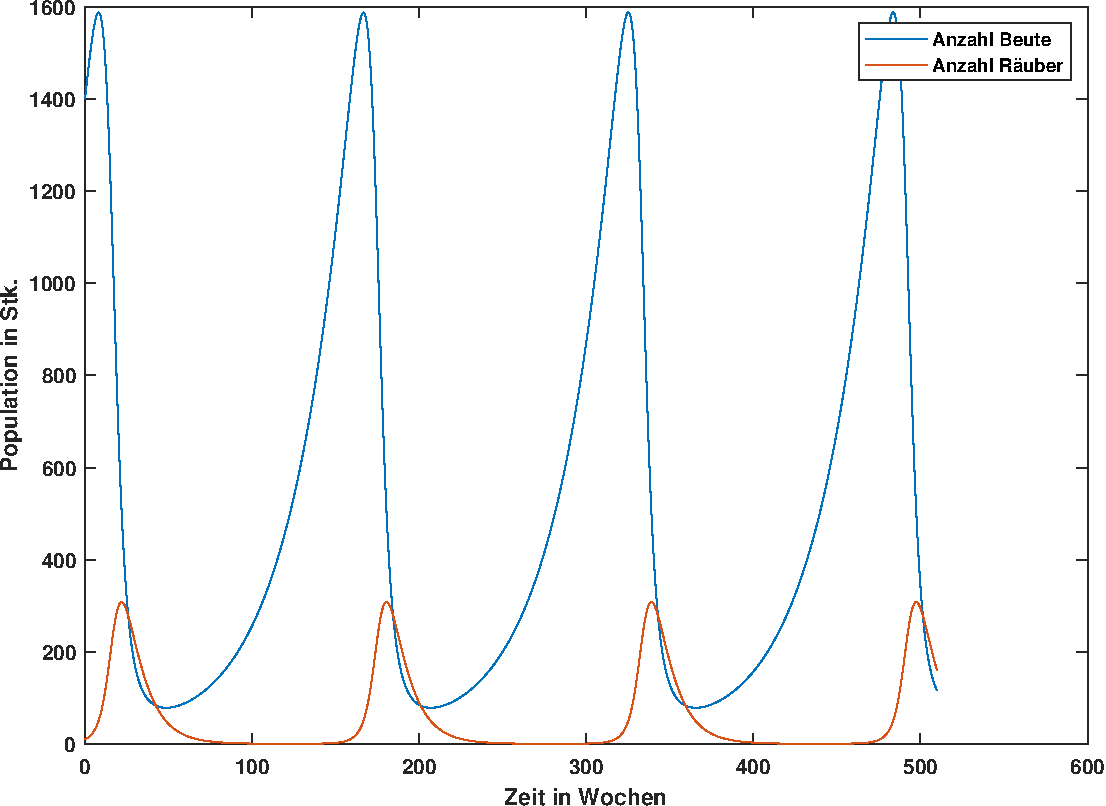
\includegraphics[width=\linewidth,height=0.8\linewidth]{fig/model/Modell1_1400_10}
		\caption{Modell \RN{1} f�r $x_{10} = 1400$ und $x_{20} = 10$}
		\label{img:haupt:mod1_1400_10}
	\end{subfigure}
	\vfill
	\begin{subfigure}[h]{0.49\linewidth}
		\centering
		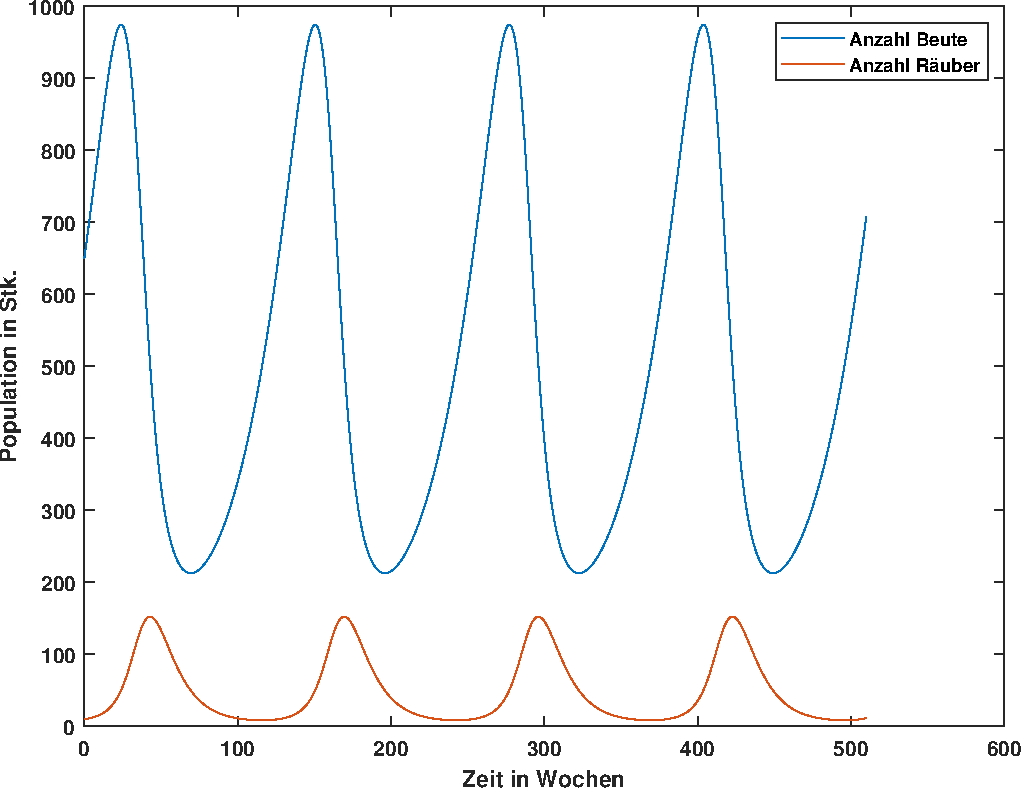
\includegraphics[width=\linewidth,height=0.8\linewidth]{fig/model/Modell1_650_10}
		\caption{Modell \RN{1} f�r $x_{10} = 650$ und $x_{20} = 10$}
		\label{img:haupt:mod1_650_10}
	\end{subfigure}
	\caption{Modell \RN{1} f�r $x_{20} = 10$ und $x_{10} = \{2500, 1400, 650\}$}
	\label{img:haupt:mod1_x10_10}
\end{figure}

\begin{figure}
	\begin{subfigure}[h]{0.49\linewidth}
		\centering
		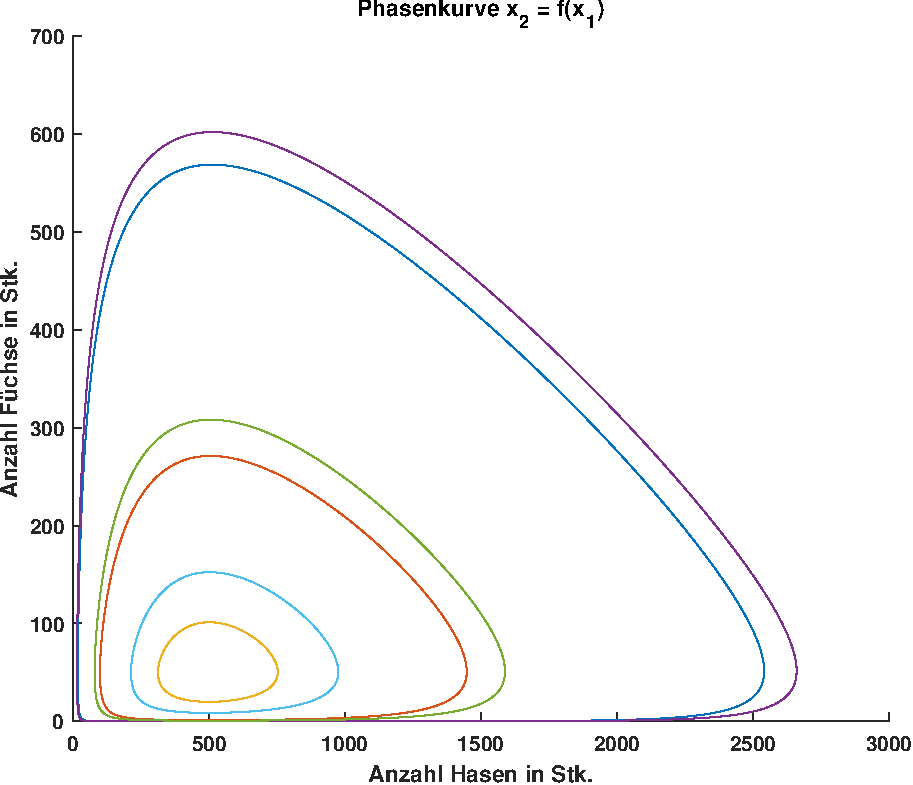
\includegraphics[width=\linewidth,height=0.8\linewidth]{fig/model/Modell1_Phase}
		\caption{Iterativ berechnete Phasenkurven}
		\label{img:haupt:mod1_phase}
	\end{subfigure}
	\hfill
	\begin{subfigure}[h]{0.49\linewidth}
		\centering
		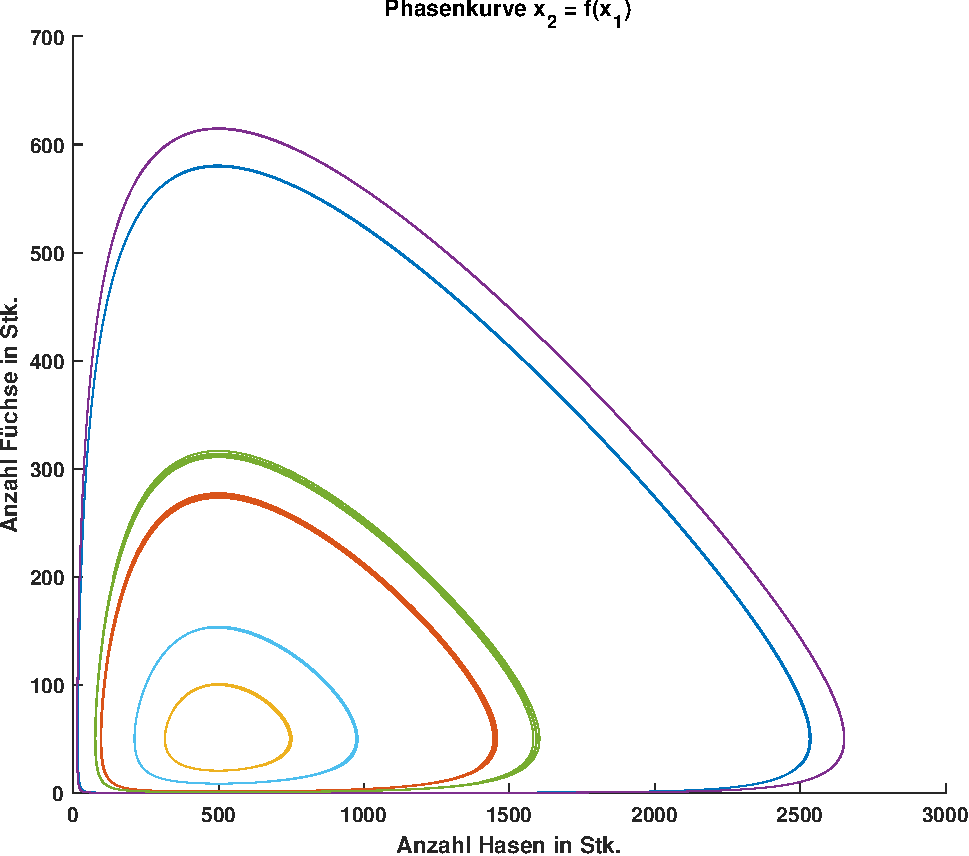
\includegraphics[width=\linewidth,height=0.8\linewidth]{fig/model/Modell1_PhaseOde}
		\caption{Phasenkurven des ode45-Solver}
		\label{img:haupt:mod1_phase_ode}
	\end{subfigure}
	\caption{Phasenkurven $x_2 = f(x_1)$ des Modell \RN{1} f�r verschiedene Anfangswerte}
	\label{img:haupt:mod1_phasen}
\end{figure}

\FloatBarrier

\FloatBarrier
\subsection{Model \RN{2}: Begrenztes Populations-Modell}
\label{sec:haupt:model2}

\subsubsection{Realisierung in MATLAB}
\label{sec:haupt:matlab2}
%Die Realisierung des Modells \RN{2}, unter Verwendung von MATLAB, ist in \autoref{lst:matlab2:code} gegeben. Die Implementierung ist, bis auf spezifische Anpassungen f�r Modell \RN{2}, weitestgehend identisch mit der Realisierung in \autoref{lst:matlab1:code}. Die Parameter $a_1, b_1, c_1, a_2$ und $b_2$ werden in einem ersten Schritt deklariert und initialisiert. Ebenso wird der Zeitvektor $t$, mithilfe der Dauer $tmax$ und dem entsprechenden Zeitschritt $dt$, erstellt. Es wird eine weitere Variable $W$ deklariert und initialisiert, mit der die Weidefl�che bzw. Kapazit�tsgrenze abgebildet werden kann.

\begin{lstlisting}[style=Matlab-editor,caption={Deklarieren und initialisieren von Parametern},captionpos=b,label=lst:matlab2:param,language=Matlab,basicstyle=\mlttfamily,numbers=none,frame=single,escapeinside={*@}{@*}]
%% Randbedingungen / Parameter [pro Woche]

% Beute / Hasen
a1 = 0.05; % Geburtenrate: Verdopplung der Population in 20 Wochen
b1 = 0.02; % Sterberate: 2% der Hasen sterben an nat�rlichen Ursachen
c1 = 0.0006; % Fressrate der F�chse

% R�uber / F�chse
a2 = 0.0002; % Geburtenrate/Beutewahrscheinlichkeit der F�chse
b2 = 0.1; % Sterberate: F�chse verlieren pro Woche 10% Biomasse

% Anfangsbedingungen
W = 1400; % Maximalzahl der Hasen
dt = 1/7; % Zeitschritt
tmax = 51*10; % Dauer in Wochen
t = 0:dt:tmax; % Zeitvektor
\end{lstlisting}

Wie in Modell \RN{1}, werden sechs Anfangszust�nde f�r $x_{10} = \{2500, 1400, 650\}$ und $x_{20} = \{25, 10\}$ in $for$-Schleifen abgebildet. Es wird f�r jeden Zeitschritt die �nderung der Beute- und R�uberpopulation berechnet. Hierbei wird die Berechnung, um die �nderung der Beutepopulation zu bestimmen, an das logistische Wachstum angepasst. Hierzu wird der Term $\frac{W - x1}{W}$ als weiterer Faktor, zur Wachstumsrate $r = a_1 - b_1$, hinzugef�gt.

\begin{lstlisting}[style=Matlab-editor,caption={Berechnen der Verl�ufe und Phasenkurven der Populationen},captionpos=b,label=lst:matlab2:calc,language=Matlab,basicstyle=\mlttfamily,numbers=none,frame=single,escapeinside={*@}{@*}]
% Eigene Axis f�r Phasenkurven
ax = gca;

%% Berechnung

for x20 = [25 10]

for x10 = [2500 1400 650]

	% mit Anfangswerten initialisieren
	x1(1) = x10;
	x2(1) = x20;
	
	for i = 2:length(t)
	
	% �nderung der Beutepopulation mit logistischem Wachstum
	dx1 = 1/W*(W-x1(i - 1))*(a1 - b1)*x1(i - 1) - c1*x2(i - 1)*x1(i - 1);
	x1(i) = x1(i - 1) + dt*dx1;
	
	% �nderung der R�uberpopulation
	dx2 = (a2*x2(i - 1)*x1(i - 1) - b2*x2(i - 1));
	x2(i) = x2(i - 1) + dt*dx2;
	
	end
	
	figure
	plot(t,x1,t,x2)
	xlabel('Zeit in Wochen','Fontweight','bold')
	ylabel('Population in Stk.','Fontweight','bold')
	legend('Anzahl Beute','Anzahl R�uber')
	set(gca,'Fontweight','bold')
	
	hold(ax,'on')
	plot(ax,x1,x2)
	hold(ax,'off')

end

end

xlabel(ax,'Anzahl Hasen in Stk.','Fontweight','bold')
ylabel(ax,'Anzahl F�chse in Stk.','Fontweight','bold')
title(ax,'Phasenkurve x_2 = f(x_1)')
set(ax,'Fontweight','bold')
\end{lstlisting}

Die Phasenkurven lassen sich, ebenso wie f�r das Modell \RN{1}, mit dem \enquote{ode45}-Solver approximieren. Hierzu wird die angepasste \autoref{eqn:haupt:logw} und \autoref{eqn:grundl:x2} in einer anonymen Funktion gespeichert. 

\begin{lstlisting}[style=Matlab-editor,caption={Bestimmung der Phasenkurven durch den ode45-Solver},captionpos=b,label=lst:matlab2:ode,language=Matlab,basicstyle=\mlttfamily,numbers=none,frame=single,escapeinside={*@}{@*}]
figure
hold on
% Zustandsdifferentialgleichungen in anonymer Funktion speichern
f = @(t,x) [x(1)*((a1 - b1)*(1/W*(W - x(1))) - c1*x(2)); x(2)*(a2*x(1) - b2)];

%Phasenkurven f�r verschiedene Anfangsbedingungen bestimmen
for x20 = [25 10]

for x10 = [2500 1400 650]

	% Verlauf mit ode45 solver berechnen
	[~, xs] = ode45(f,t, [x10, x20]);
	% Phasenkurve plotten
	plot(xs(:,1), xs(:,2))

end

end

xlabel('Anzahl Hasen in Stk.','Fontweight','bold')
ylabel('Anzahl F�chse in Stk.','Fontweight','bold')
title('Phasenkurve x_2 = f(x_1)')
set(gca,'Fontweight','bold')
hold off
\end{lstlisting}

\FloatBarrier

Die Verl�ufe der Populationen sind in \autoref{img:haupt:mod2_2500_25} bis \autoref{img:haupt:mod2_650_10} dargestellt. Die entsprechenden Schwankungen der Populationen werden, durch die begrenzte Weidefl�che, ged�mpft. Es ist zu beobachten, dass beide Populationen gegen jeweils einen bestimmten Endwert konvergieren. Dieser ist unabh�ngig von den entsprechenden Anfangszust�nden. Hierauf wird in \autoref{sec:haupt:stationaer} n�her eingegangen. Es ist ebenfalls zu beobachten, dass die Beutepopulation f�r $x_1 \geq W$ rapide abf�llt. Hierbei ist die Kapazit�tsgrenze der Weidefl�che erreicht und es stehen nicht genug Ressourcen f�r alle Beutetiere zur Verf�gung. F�r den Fall $x_{10} = 650$ und $x_{20} = 10$ in \autoref{img:haupt:mod2_650_10} ist, da hierbei $x_1 < W$ gilt, ein Wachstum der Beutepopulation m�glich und zu verzeichnen.
\\
\\
Die Phasenkurven der Anfangszust�nde $x_{10} = \{2500, 1400, 650\}$ und $x_{20} = \{25, 10\}$ f�r das Modell \RN{2} sind in \autoref{img:haupt:mod2_phasen} dargestellt. Hierbei sind keine wesentlichen Unterschiede zwischen der iterativen Berechnung der Phasenkurven und der Bestimmung durch den \enquote{ode45}-Solver zu verzeichnen. Im Gegensatz zu den Phasenkurven f�r das Modell \RN{1} in \autoref{img:haupt:mod1_phase} ist es schwieriger genauere Aussagen �ber den Einfluss der Anfangszust�nde zu machen. Der Verlauf der Phasenkurven ist hierbei wesentlich komplexer. Es ist jedoch das Konvergenzverhalten aller Phasenkurven in Richtung eines station�ren Zustands anzumerken, der unabh�ngig von den Anfangszust�nden ist.

\begin{figure}
	\centering
	\begin{subfigure}[h]{0.49\linewidth}
		\centering
		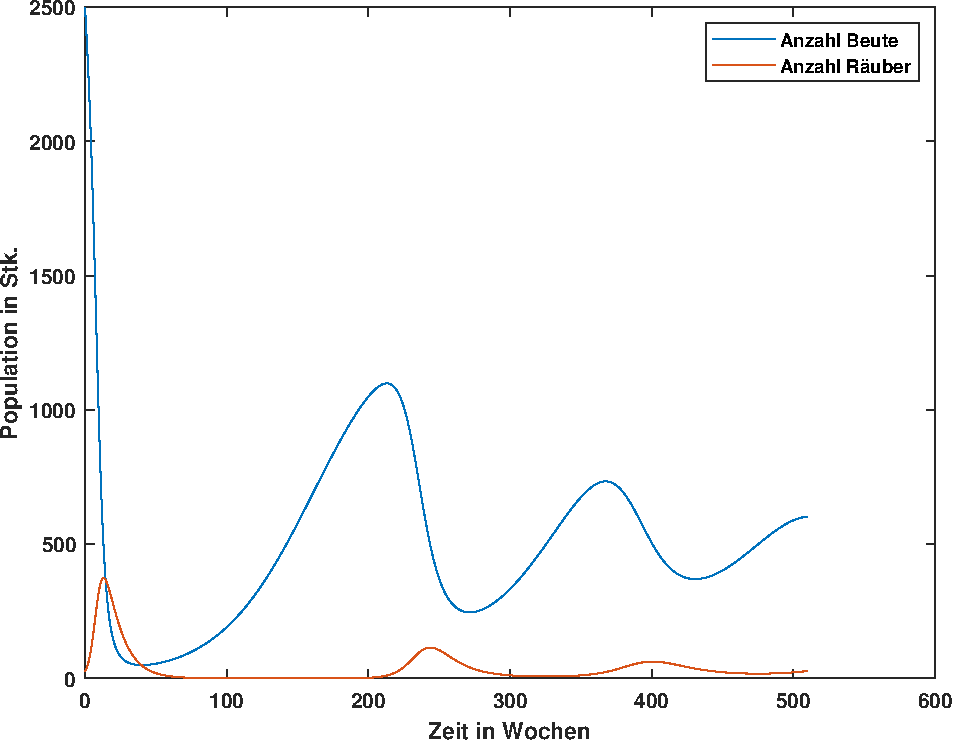
\includegraphics[width=\linewidth,height=0.8\linewidth]{fig/model/Modell2_2500_25}
		\caption{Modell \RN{2} f�r $x_{10} = 2500$ und $x_{20} = 25$}
		\label{img:haupt:mod2_2500_25}
	\end{subfigure}
	\hfill
	\begin{subfigure}[h]{0.49\linewidth}
		\centering
		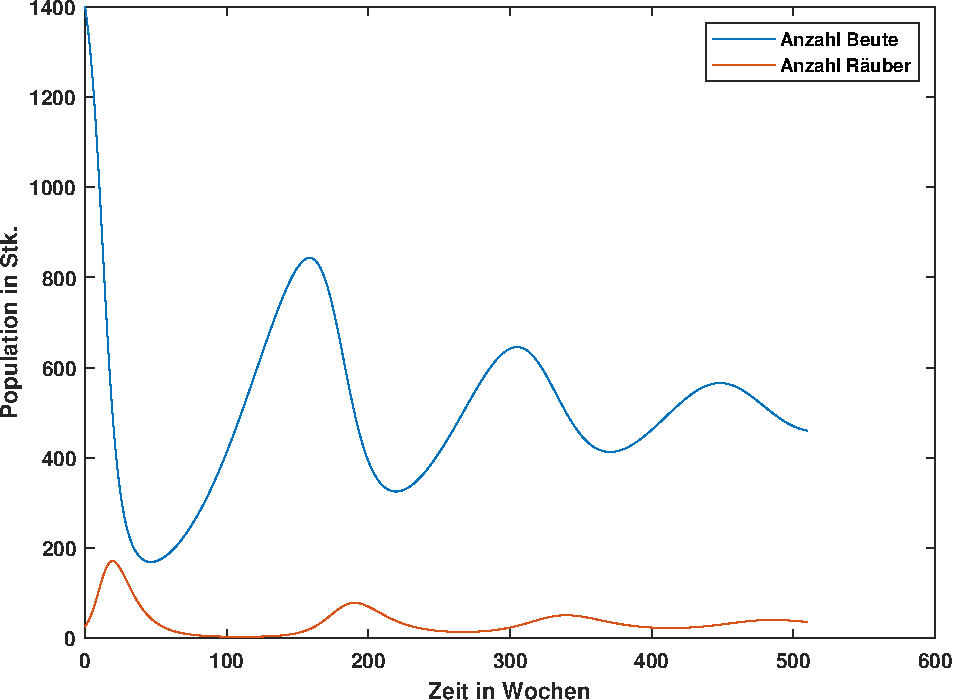
\includegraphics[width=\linewidth,height=0.8\linewidth]{fig/model/Modell2_1400_25}
		\caption{Modell \RN{2} f�r $x_{10} = 1400$ und $x_{20} = 25$}
		\label{img:haupt:mod2_1400_25}
	\end{subfigure}
	\vfill
	\begin{subfigure}[h]{0.49\linewidth}
		\centering
		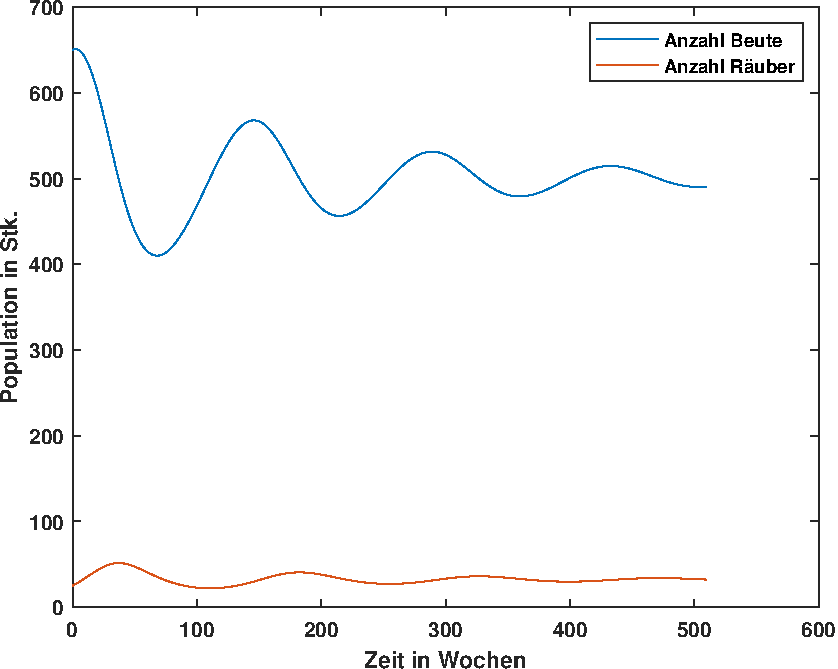
\includegraphics[width=\linewidth,height=0.8\linewidth]{fig/model/Modell2_650_25}
		\caption{Modell 2 f�r $x_{10} = 650$ und $x_{20} = 25$}
		\label{img:haupt:mod2_650_25}
	\end{subfigure}
	\caption{Modell \RN{2} f�r $x_{20} = 25$ und $x_{10} = \{2500, 1400, 650\}$}
	\label{img:haupt:mod2_x10_25}
\end{figure}

\begin{figure}
	\centering
	\begin{subfigure}[h]{0.49\linewidth}
		\centering
		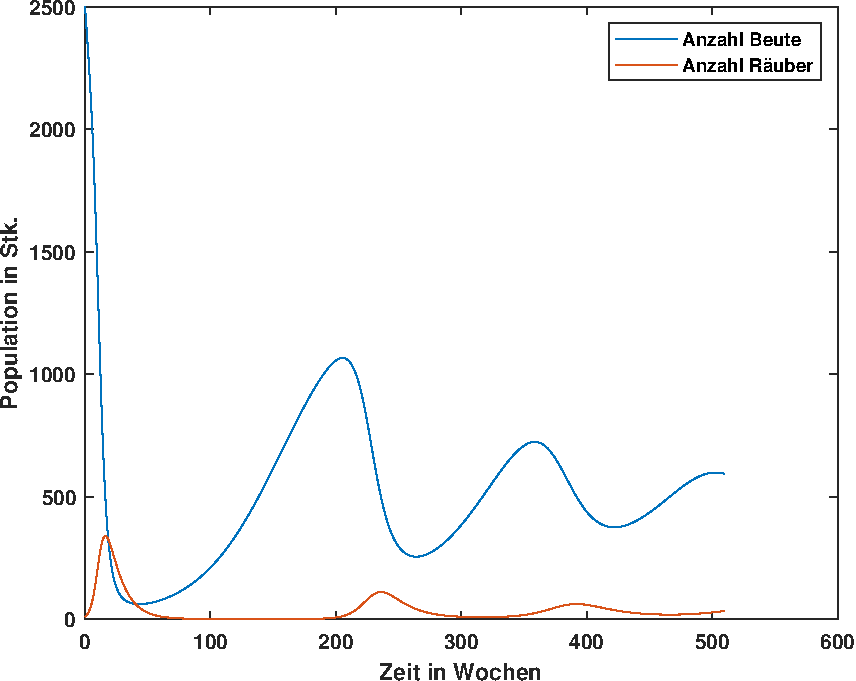
\includegraphics[width=\linewidth,height=0.8\linewidth]{fig/model/Modell2_2500_10}
		\caption{Modell \RN{2} f�r $x_{10} = 2500$ und $x_{20} = 10$}
		\label{img:haupt:mod2_2500_10}
	\end{subfigure}
	\hfill
	\begin{subfigure}[h]{0.49\linewidth}
		\centering
		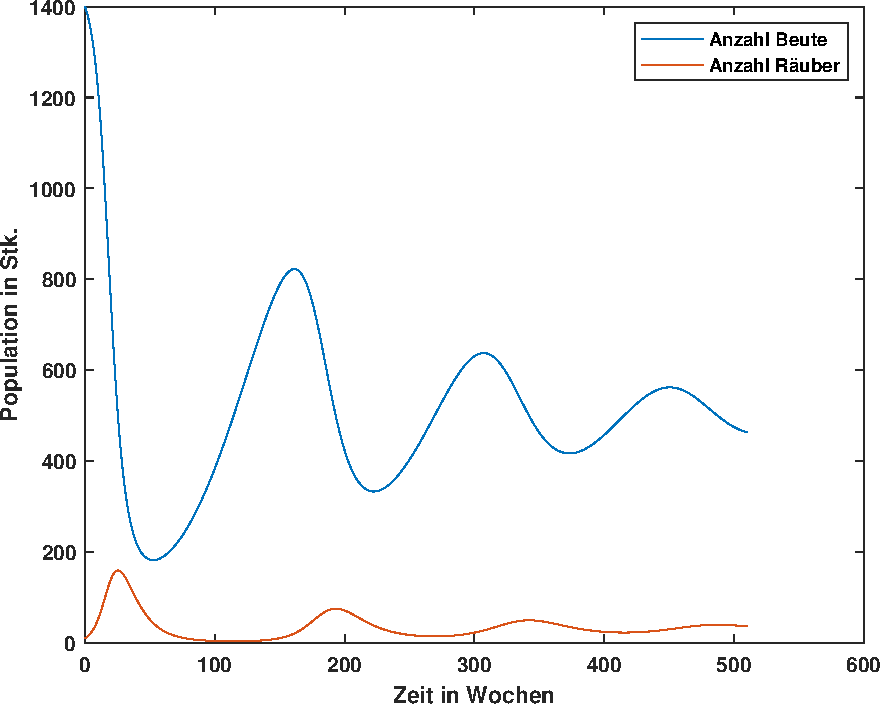
\includegraphics[width=\linewidth,height=0.8\linewidth]{fig/model/Modell2_1400_10}
		\caption{Modell \RN{2} f�r $x_{10} = 1400$ und $x_{20} = 10$}
		\label{img:haupt:mod2_1400_10}
	\end{subfigure}
	\vfill
	\begin{subfigure}[h]{0.49\linewidth}
		\centering
		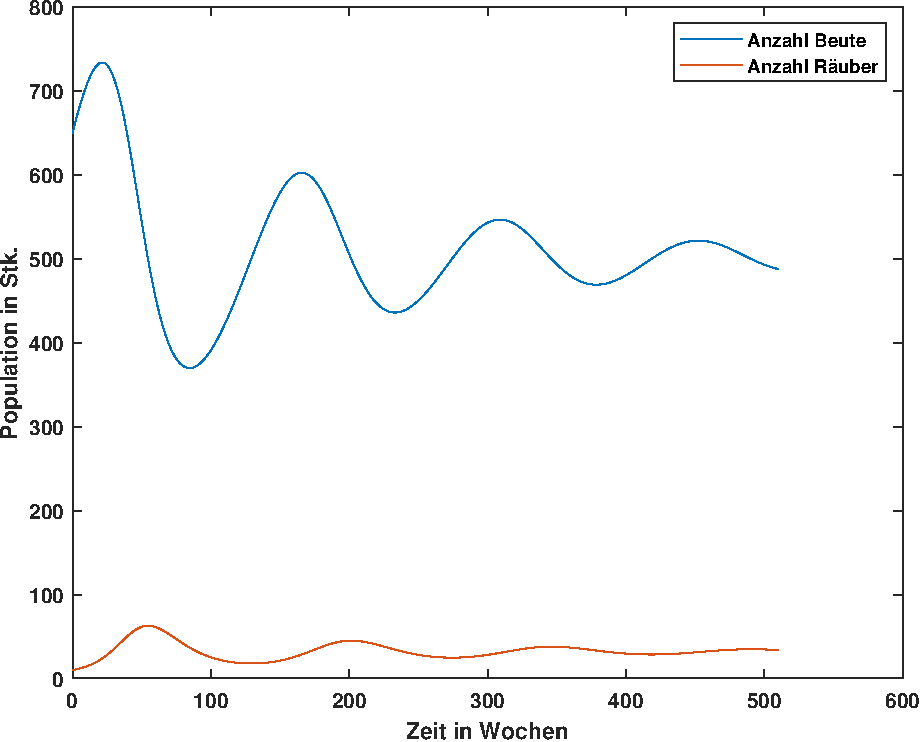
\includegraphics[width=\linewidth,height=0.8\linewidth]{fig/model/Modell2_650_10}
		\caption{Modell \RN{2} f�r $x_{10} = 650$ und $x_{20} = 10$}
		\label{img:haupt:mod2_650_10}
	\end{subfigure}
	\caption{Modell \RN{2} f�r $x_{20} = 10$ und $x_{10} = \{2500, 1400, 650\}$}
	\label{img:haupt:mod2_x10_10}
\end{figure}


\begin{figure}
	\begin{subfigure}[h]{0.49\linewidth}
		\centering
		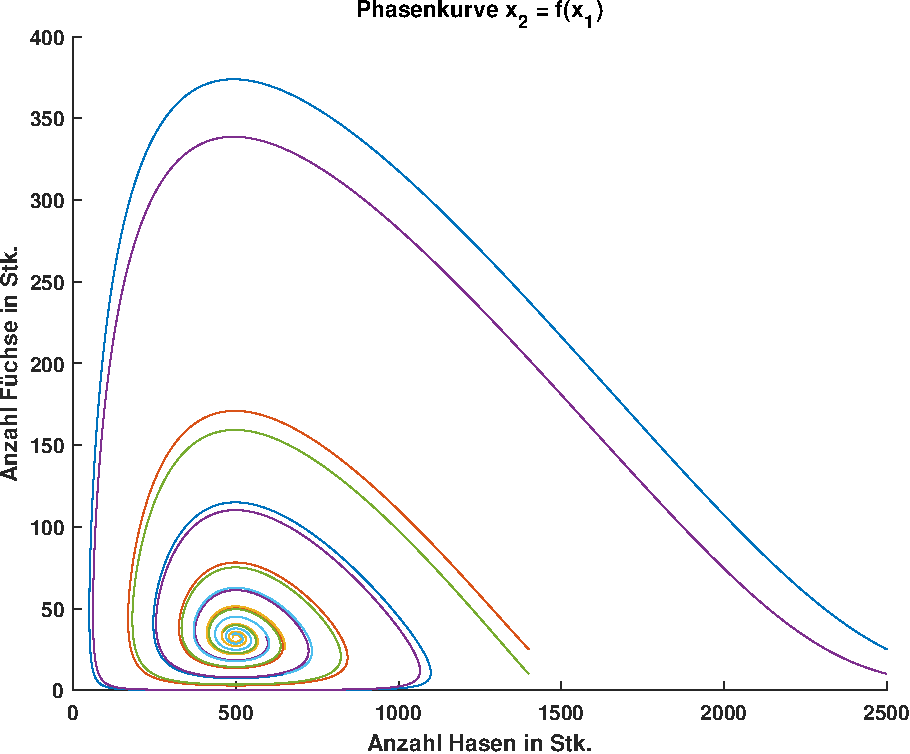
\includegraphics[width=\linewidth,height=0.8\linewidth]{fig/model/Modell2_Phase}
		\caption{Iterativ berechnete Phasenkurven}
		\label{img:haupt:mod2_phase}
	\end{subfigure}
	\hfill
	\begin{subfigure}[h]{0.49\linewidth}
		\centering
		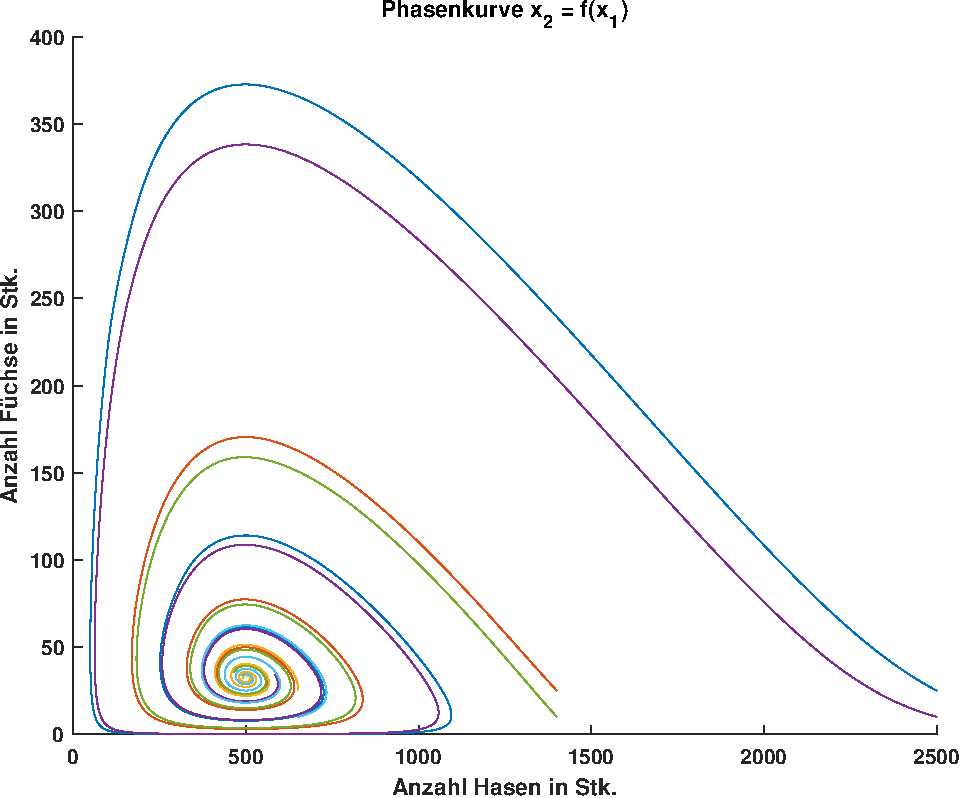
\includegraphics[width=\linewidth,height=0.8\linewidth]{fig/model/Modell2_PhaseOde}
		\caption{Phasenkurven des ode45-Solver}
		\label{img:haupt:mod2_phase_ode}
	\end{subfigure}
	\caption{Phasenkurven $x_2 = f(x_1)$ des Modell \RN{2} f�r verschiedene Anfangswerte}
	\label{img:haupt:mod2_phasen}
\end{figure}

\FloatBarrier

\FloatBarrier
\subsection{Experimente}
\label{sec:haupt:experimente}

\subsubsection{Ermittlung des station�ren Zustands}
\label{sec:haupt:stationaer}
%F�r das Modell \RN{2} war ein Konvergenzverhalten der Populationen zu beobachten. Diese konvergieren in Richtung eines station�ren Zustands. Sie werden auch als Ruhe- bzw. Gleichgewichtslagen $G$, des Lotka-Volterra-Modells, bezeichnet. Sie sind dadurch charakterisiert, dass keine zeitlichen Ver�nderungen der Zustandsvariablen mehr stattfinden \cite[S. 32]{lit:Foellinger1982}:

\begin{align*}
	\dot{x}_1 = 0, \qquad \dot{x}_2 = 0
\end{align*}

Damit folgt aus \autoref{eqn:grundl:x1} und \autoref{eqn:grundl:x2} \cite[S. 32]{lit:Foellinger1982}:

\begin{align}
	(a_1 - b_1 - c_1x_2)x_1 &= 0 
	\label{eqn:haupt:statx1} \\
	(a_2x_1 - b_2)x_2 &= 0
	\label{eqn:haupt:statx2}
\end{align}

Daraus ergibt sich zun�chst die triviale L�sung

\begin{align*}
	x_1 = 0, \qquad x_2 = 0
\end{align*}

in dem die R�uber sowie die Beute ausgestorben sind. Um den weiteren station�ren Zustand der Populationen zu bestimmen, m�ssen die beiden Ausdr�cke in den Klammern in \autoref{eqn:haupt:statx1} und \autoref{eqn:haupt:statx2} null werden \cite[S. 33]{lit:Foellinger1982}:

\begin{align}
	a_1 - b_1 - c_1x_2 &= 0
	\label{eqn:haupt:statx12} \\
	a_2x_1 - b_2 &= 0\
	\label{eqn:haupt:statx22} \
\end{align}

Daraus folgt, f�r die Zustandsvariablen $x_1$ und $x_2$, die Ruhelage $G$ \cite[S. 33]{lit:Foellinger1982}:

\begin{align}
	x_{1G} &= \frac{b_2}{a_2}
	\label{eqn:haupt:x1g} \\
	x_{2G} &= \frac{a_1 - b_1}{c_1}
	\label{eqn:haupt:x2g}
\end{align}

In dieser Gleichgewichtslage entspricht der Zuwachs an Beutetieren der Anzahl an durch die R�uber aufgezehrten Tiere. Ebenso bleibt die R�uberpopulation konstant. Da sich die Anzahl beider Populationen nicht �ndert, stellt die Gleichgewichtslage eine spezielle Trajektorie dar. Diese entspricht, wie in \autoref{img:haupt:phaseG} dargestellt, einem Punkt.

\begin{figure}
	\centering
	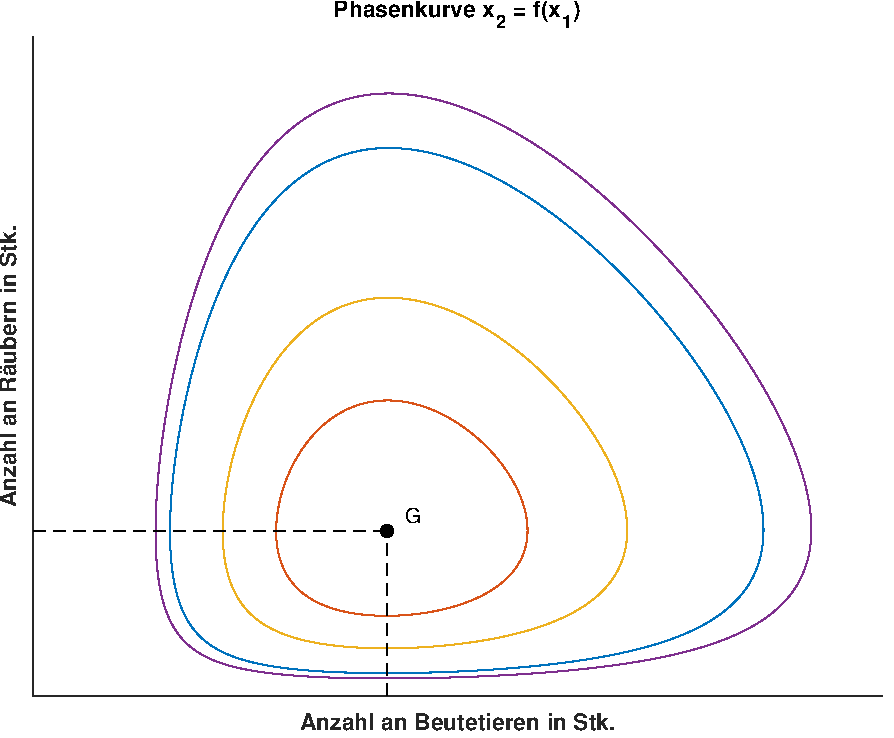
\includegraphics[width=0.6\linewidth,height=0.5\linewidth]{fig/exp/phaseG}
	\caption{Gleichgewichtslage in der Zustandsebene}
	\label{img:haupt:phaseG}
\end{figure}

Es ist anzumerken, dass die in \autoref{eqn:haupt:x1g} und \autoref{eqn:haupt:x2g} angegebenen Gleichgewichtslagen f�r $x_1$ und $x_2$ nicht von den Anfangspunkten abh�ngig sind. Diese Anfangspunkte bestimmen nur die entsprechende Trajektorie in der Zustandsebene. Die Ruhelage ist ausschlie�lich von den, in \autoref{sec:grundl:gl} genannten und beschriebenen, Faktoren $a_1, b_1, c_1, a_2,$ und $b_2$ abh�ngig. Diese beschreiben die entsprechenden Wechselwirkungen innerhalb und zwischen den Populationen. F�r die in \autoref{tab:haupt:param} gegebenen Werte, ergibt sich folgende Gleichgewichtslage:

\begin{align}
	x_{1G} &= \frac{b_2}{a_2} = \frac{0.1}{0.0002} = 500 \\
	x_{2G} &= \frac{(a_1 - b_1)}{c_1} = \frac{(0.05 - 0.02)}{0.0006} = 50
\end{align}

Eine M�glichkeit, die Gleichgewichtslage zu bestimmen, ist es diese numerisch zu approximieren. Hierzu wird in \autoref{lst:stat:code1} die Funktion $fsolve()$ verwendet. \autoref{eqn:haupt:statx12} und \autoref{eqn:haupt:statx22} werden, mit den entsprechenden Parametern $a_1, b_1, c_1, a_2$ und $b_2$, in einer anonymen Funktion gespeichert. Diese wird $fsolve()$ mit entsprechenden Startbedingungen �bergeben und anschlie�end die Gleichung $f = 0$ approximiert.

\begin{lstlisting}[style=Matlab-editor,caption={Verwenden von fsolve() f�r das numerische Bestimmen der Gleichgewichtslage},captionpos=b,label=lst:stat:code1,language=Matlab,basicstyle=\mlttfamily,numbers=none,frame=single,escapeinside={*@}{@*}]
% Parameter

% Beute / Hasen
a1 = 0.1; % Geburtenrate
b1 = 0.02; % Sterberate
c1 = 0.002; % Fressrate

% R�uber / F�chse
a2 = 0.0004; % Geburtenrate
b2 = 0.2; % Sterberate

% Deklarieren symbolischer Variablen
syms x1 x2
% Deklarieren der Gleichungen, um die Gleichgewichtslage zu bestimmen
f = @(x) [(a1 - b1 - c1*x(2));(a2*x(1) - b2)];
% Numerisches L�sen der Gleichungen mithilfe von vpasolve()
x = fsolve(f,[10,10])
\end{lstlisting}

Eine weitere M�glichkeit, die Gleichgewichtslage numerisch zu approximieren, ist mit der MATLAB Funktion $vpasolve()$ m�glich. In \autoref{lst:stat:code2} ist die Vorgehensweise hierzu exemplarisch dargestellt. In einem ersten Schritt werden hierbei die Parameter $a_1, b_1, c_1, a_2$ und $b_2$ deklariert und mit den in \autoref{tab:haupt:param} gegebenen Werten initialisiert. Anschlie�en werden, f�r die Zustandsvariablen $x_1$ und $x_2$, zwei symbolische Variablen mithilfe des \enquote{syms}-Befehls deklariert. Diese werden dazu verwendet, um \autoref{eqn:haupt:statx12} und \autoref{eqn:haupt:statx22}, unter Verwendung der symbolischen Variablen, in MATLAB zu definieren. Die definierten Gleichungen werden anschlie�end, mit der entsprechenden symbolischen Variablen, nach der die Gleichung aufgel�st werden soll, der Funktion $vpasolve()$ �bergeben. Diese approximiert numerisch N�herungswerte f�r $x_{1G}$ bzw. $x_{2G}$ und liefert die Ann�herungsl�sungen als R�ckgabewert.
\begin{lstlisting}[style=Matlab-editor,caption={Verwenden von vpasolve() f�r das numerische Bestimmen der Gleichgewichtslage},captionpos=b,label=lst:stat:code2,language=Matlab,basicstyle=\mlttfamily,numbers=none,frame=single,escapeinside={*@}{@*}]
% Parameter

% Beute / Hasen
a1 = 0.1; % Geburtenrate
b1 = 0.02; % Sterberate
c1 = 0.002; % Fressrate

% R�uber / F�chse
a2 = 0.0004; % Geburtenrate
b2 = 0.2; % Sterberate

% Deklarieren symbolischer Variablen
syms x1 x2
% Deklarieren der Gleichungen, um die Gleichgewichtslage zu bestimmen
eqnx1 = a1 - b1 - c1*x2 == 0;
eqnx2 = a2*x1 - b2 == 0;
% Numerisches L�sen der Gleichungen mithilfe von vpasolve()
% Erste Gleichung nach x2 aufl�sen
x2G = vpasolve(eqnx1, x2);
% Zweite Gleichung nach x1 aufl�sen
x1G = vpasolve(eqnx2, x1);
\end{lstlisting}

\FloatBarrier

\subsubsection{Einfluss eines einmaligen Eingriffs}
\label{sec:haupt:eingriff}
%Nachfolgend wird beschrieben, wie sich ein einmaliger Eingriff, beispielsweise durch Halbierung der R�uberpopulation, auf die Populationen auswirken kann. Dies ist beispielsweise eine wichtige Fragestellung in dem Bereich der Landwirtschaft. Hierbei k�nnen sch�dliche Insekten als Beute und Parasiten, die sich von den Insekten ern�hren, als R�uber interpretiert werden. Beide dieser Populationen sind Sch�dlinge, die in der Landwirtschaft bek�mpft werden. Hierbei stellt sich die Frage welcher Zeitpunkt, w�hrend des periodischen Bio-Zyklus, als g�nstig angesehen wird, um die Populationen zu verringern oder vernichten. Ein Eingreifen zu einem ung�nstigen Zeitpunkt kann die momentane Trajektorie in eine andere mit einer weitaus h�heren Schwankungen der Populationen transformieren. \cite[S. 35 f.]{lit:Foellinger1982}
\\
\\
Um einen passenden Zeitpunkt f�r die Sch�dlingsbek�mpfung treffen zu k�nnen, werden zun�chst die Phasenkurven in \autoref{img:haupt:phaseE} und die entsprechende Gleichgewichtslage analysiert. Die folgenden Geraden schneiden den station�ren Zustand und teilen die Zustandsebene in vier Subquadranten \cite[S. 7]{lit:Helmreich2011}:

\begin{align}
	x_2 &= \frac{(a_1 - b_1)}{c_1} 
	\label{eqn:haupt:x2E} \\
	x_1 &= \frac{a_2}{b_2}
	\label{eqn:haupt:x1E}
\end{align}

Der erste Subquadrant ist durch $x_2 \leq \frac{a_1 - b_1}{c_1}$ und $x_1 \leq \frac{a_2}{b_2}$ definiert. Dieser Teilbereich der Phasenkurven ist dadurch gekennzeichnet, dass sich die Anzahl an R�ubern $x_2$ verringert, w�hrend sich die Beutepopulation $x_1$ erh�ht. Eine Halbierung der R�uberpopulation $x_2$ hat hierbei die Transformation in eine Trajektorie mit einem gr��eren Umfang zur Folge. Die Schwankungen der beiden Populationen w�rden in diesem Fall zunehmen.
\\
\\
In dem zweiten Subquadranten gelten f�r $x_1 > \frac{a_2}{b_2}$ und $x_2 \leq \frac{a_1 - b_1}{c_1}$. Hierbei steigen beide Populationen an. \\Eine Halbierung der R�uber in diesem Subquadranten hat, wie im ersten Fall, eine Erh�hung der beiden Populationen zur Folge.
\\
\\
Der dritte Subquadrant ist durch $x_1 > \frac{a_2}{b_2}$ und $x_2 > \frac{a_1 - b_1}{c_1}$ definiert. Die Beutepopulation nimmt hierbei ab, w�hrend die R�uber sich vermehren. Eine Verringerung der R�uberpopulation hat, in diesem Fall, eine Verminderung beider Populationen zur Folge. Es erfolgt hierbei eine Transformation in eine der Gleichgewichtslage n�her gelegenen Trajektorie, die einen geringeren Umfang und somit geringere Schwankungen der Populationen aufweist. 
\\
\\
In dem vierten Subquadranten ist die Beutepopulation $x_1 \leq \frac{a_2}{b_2}$ und die Anzahl der R�uber $x_2 > \frac{a_1 - b_1}{c_1}$. In diesem Teilbereich verringern sich beide Populationen. Eine Verminderung der R�uber hat, wie f�r den dritten Subquadranten, eine Transformation in eine der Gleichgewichtslage n�her gelegenen Trajektorie zur Folge. Die Schwankungen der Populationen verringern sich ebenso f�r diesen Subquadranten.
\\
\\
Durch diese Fallunterscheidung l�sst sich auf einen g�nstigen Zeitpunkt schlie�en, um die R�uberpopulation dauerhaft zu verringern. Wenn diese bei einer Anzahl von $x_2 \geq 2 \cdot \frac{a_1 - b_1}{c_1}$ halbiert wird, resultiert dies in einer Transformation der momentanen Trajektorie in eine der Gleichgewichtslage n�her gelegenen Phasenkurve. Der neue Verlauf des Bio-Zyklus ist durch geringere Schwankungen der Populationen charakterisiert. Dies ist unabh�ngig von der aktuellen Beutepopulation $x_1$.

\begin{figure}
	\centering
	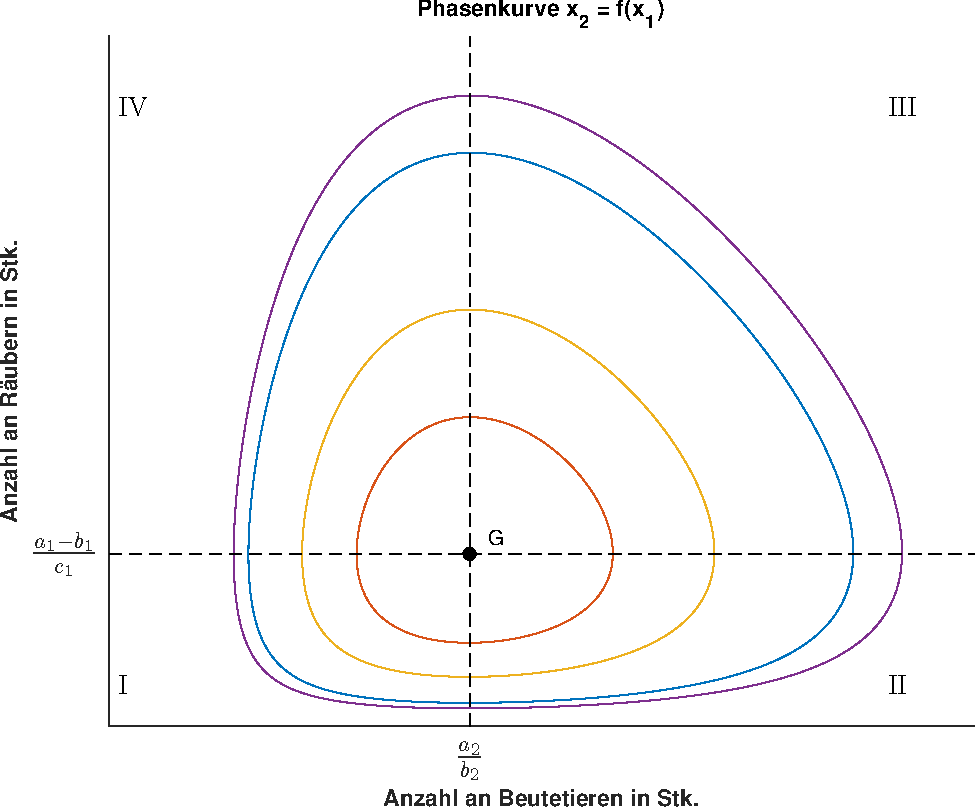
\includegraphics[width=0.6\linewidth,height=0.5\linewidth]{fig/exp/phaseE}
	\caption{Subquadranten der Trajektorien}
	\label{img:haupt:phaseE}
\end{figure}

In \autoref{img:haupt:eingriffs} sind die Auswirkungen eines Eingriffs, zu einem ung�nstigem Zeitpunkt, dargestellt. Eine Halbierung des Fuchsbestandes f�hrt hierbei zu einer Ver�nderung der Trajektorie. Die Transformation der Phasenkurve ist in \autoref{img:haupt:phaseEs} aufgezeigt. Die neue Trajektorie besitzt einen h�heren Umfang. Daraus folgt eine Zunahme an Schwankungen der Populationen. In \autoref{img:haupt:modellEs} sind diese dargestellt. Nach dem Eingriff sind gr��ere Amplituden w�hrend des periodischen Verlaufs zu vermerken.

\begin{figure}
	\begin{subfigure}[h]{0.49\linewidth}
		\centering
		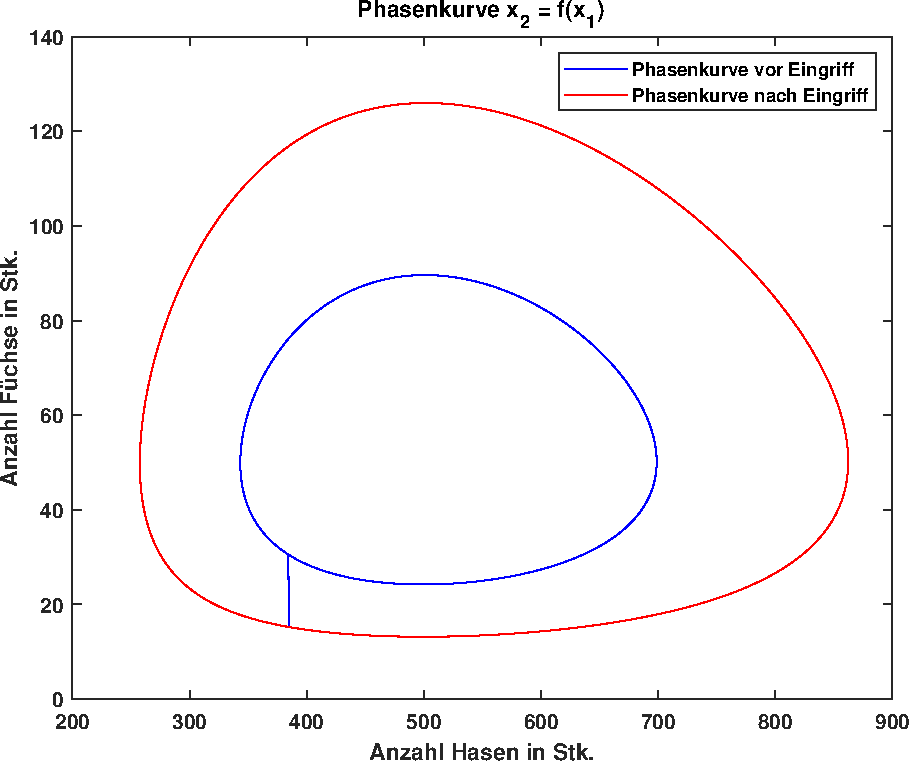
\includegraphics[width=\linewidth,height=0.8\linewidth]{fig/exp/phaseEs}
		\caption{Phasenkurve}
		\label{img:haupt:phaseEs}
	\end{subfigure}
	\hfill
	\begin{subfigure}[h]{0.49\linewidth}
		\centering
		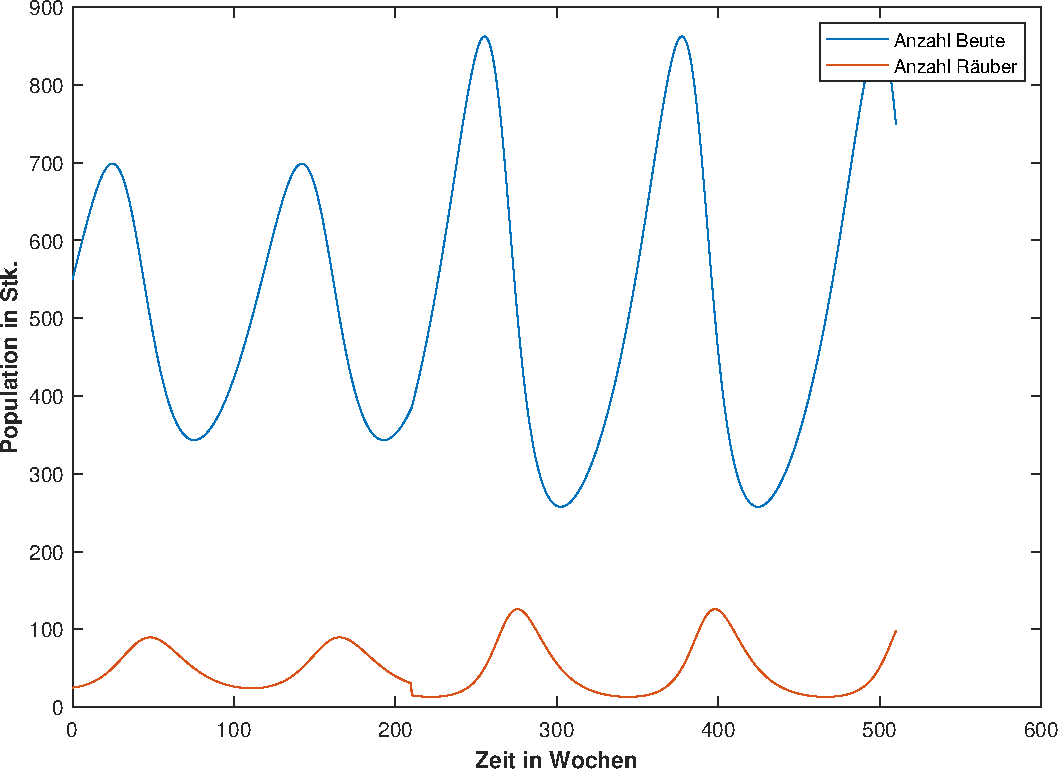
\includegraphics[width=\linewidth,height=0.8\linewidth]{fig/exp/modellEs}
		\caption{Verlauf der Populationen}
		\label{img:haupt:modellEs}
	\end{subfigure}
	\caption{Auswirkungen eines Eingriff zu einem ung�nstigem Zeitpunkt}
	\label{img:haupt:eingriffs}
\end{figure}

In \autoref{img:haupt:eingrifff} sind die gew�nschten Auswirkungen eines Eingriffs dargestellt. In \autoref{img:haupt:phaseEf} ist die Transformation in eine, der Gleichgewichtslage n�her gelegenen, Trajektorie zu erkennen. Daraus folgt ein stabilerer Verlauf der Populationen. Die Schwankungen bzw. Amplitude des periodischen Verlaufs ist hierbei, f�r beide Populationen, geringer.

\begin{figure}
	\begin{subfigure}[h]{0.49\linewidth}
		\centering
		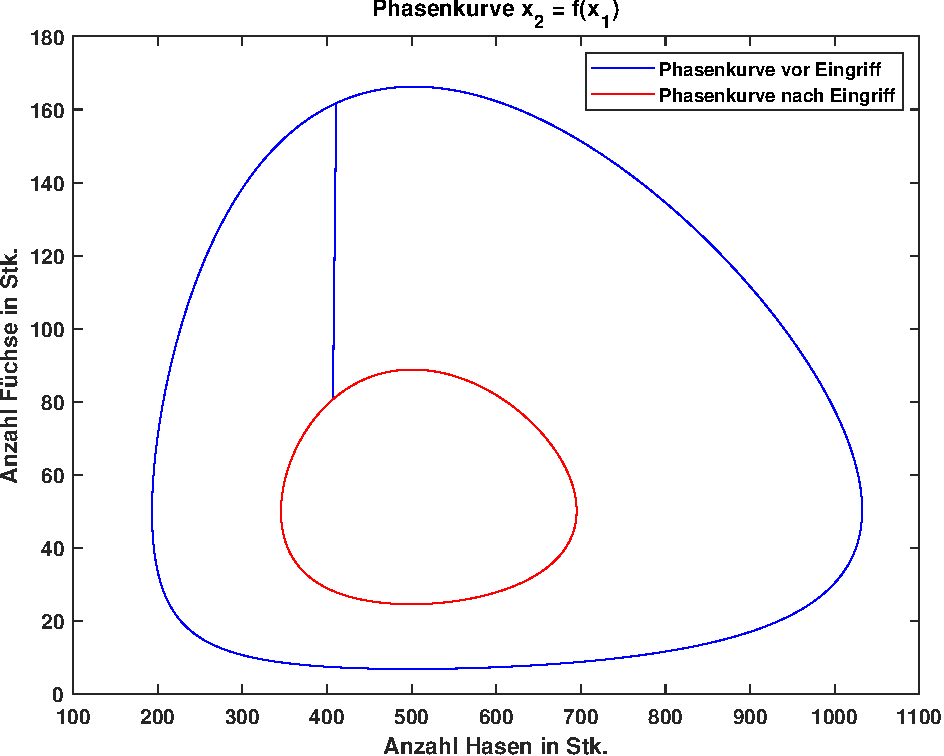
\includegraphics[width=\linewidth,height=0.8\linewidth]{fig/exp/phaseEf}
		\caption{Phasenkurve}
		\label{img:haupt:phaseEf}
	\end{subfigure}
	\hfill
	\begin{subfigure}[h]{0.49\linewidth}
		\centering
		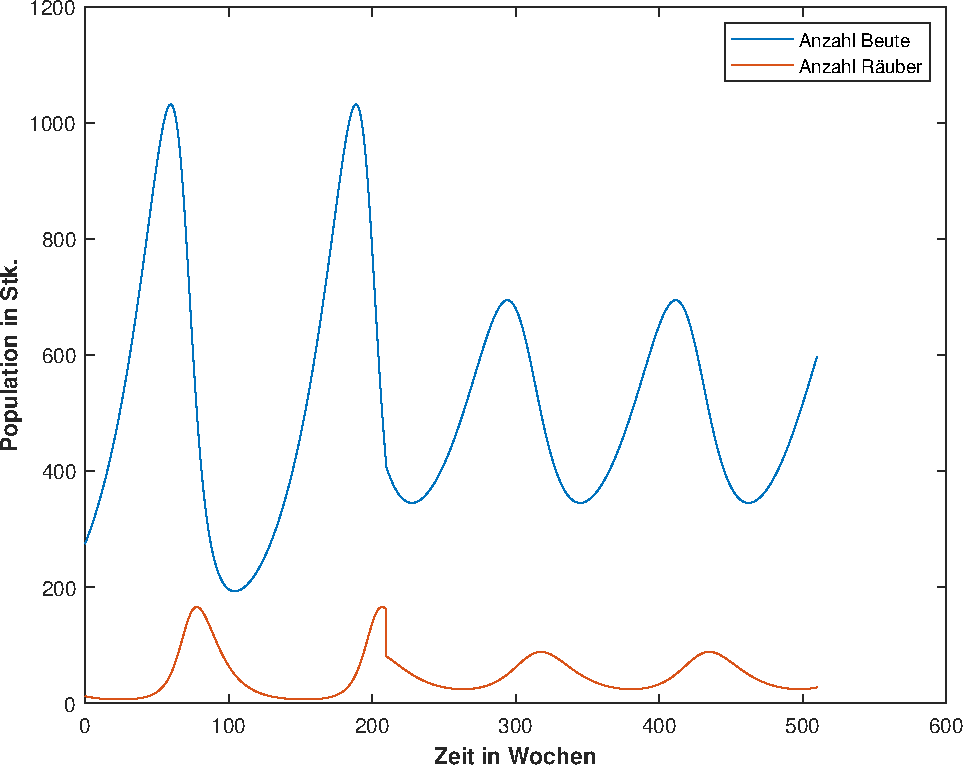
\includegraphics[width=\linewidth,height=0.8\linewidth]{fig/exp/modellEf}
		\caption{Verlauf der Populationen}
		\label{img:haupt:modellEf}
	\end{subfigure}
	\caption{Auswirkungen eines Eingriff zu einem g�nstigem Zeitpunkt}
	\label{img:haupt:eingrifff}
\end{figure}



\FloatBarrier


\section{Schluss}
\label{sec:end:intro} 

\subsection{Zusammenfassung}
\label{sec:end:zsm}

\subsection{Kritik und Ausblick}
\label{sec:end:outro}

%\appendix
%\section{Anhang}
\label{sec:a:intro}

\subsection{MATLAB Listings}
\label{sec:a:matlab}

\begin{lstlisting}[style=Matlab-editor,caption={MATLAB Code f�r das Modell 1},captionpos=b,label=lst:matlab1:code,language=Matlab,basicstyle=\mlttfamily,numbers=none,frame=single,escapeinside={*@}{@*}]
%% Randbedingungen / Parameter [pro Woche]

% Beute / Hasen
a1 = 0.05; % Geburtenrate: Verdopplung der Population in 20 Wochen
b1 = 0.02; % Sterberate: 2% der Hasen sterben an nat�rlichen Ursachen
c1 = 0.0006; % Fressrate der F�chse

% R�uber / F�chse
a2 = 0.0002; % Geburtenrate/Beutewahrscheinlichkeit der F�chse
b2 = 0.1; % Sterberate: F�chse verlieren pro Woche 10% Biomasse

% Anfangsbedingungen
dt = 1/7; % Zeitschritt
tmax = 51*10; % Dauer in Wochen
t = 0:dt:tmax; % Zeitvektor

% Eigene Axis f�r Phasenkurven
ax = gca;

%% Berechnung
for x20 = [25 10]

for x10 = [2500 1400 650]

	% mit Anfangswerten initialisieren
	x1(1) = x10;
	x2(1) = x20;
	
	for i = 2:length(t)
	
	% �nderung der Beutepopulation
	dx1 = a1*x1(i - 1) - b1*x1(i - 1) - c1*x2(i - 1)*x1(i - 1);
	x1(i) = x1(i - 1) + dt*dx1;
	
	% �nderung der R�uberpopulation
	dx2 = a2*x2(i - 1)*x1(i) - b2*x2(i - 1);
	x2(i) = x2(i - 1) + dt*dx2;
	
	end
	
	figure
	plot(t,x1,t,x2)
	xlabel('Zeit in Wochen','Fontweight','bold')
	ylabel('Population in Stk.','Fontweight','bold')
	legend('Anzahl Beute','Anzahl R�uber')
	set(gca,'Fontweight','bold')
	
	hold(ax,'on')
	plot(ax,x1,x2)
	hold(ax,'off')

end

end

xlabel(ax,'Anzahl Hasen in Stk.','Fontweight','bold')
ylabel(ax,'Anzahl F�chse in Stk.','Fontweight','bold')
title(ax,'Phasenkurve x_2 = f(x_1)')
set(ax,'Fontweight','bold')

figure
hold on
% Zustandsdifferentialgleichungen in anonymer Funktion speichern
f = @(t,x) [x(1)*(a1 - b1 - c1*x(2)); x(2)*(a2*x(1) - b2)];

%Phasenkurven f�r verschiedene Anfangsbedingungen bestimmen
for x20 = [25 10]

for x10 = [2500 1400 650]

	% Verlauf mit ode45 solver berechnen
	[~, xs] = ode45(f,t, [x10, x20]);
	% Phasenkurve plotten
	plot(xs(:,1), xs(:,2))

end

end

xlabel('Anzahl Hasen in Stk.','Fontweight','bold')
ylabel('Anzahl F�chse in Stk.','Fontweight','bold')
title('Phasenkurve x_2 = f(x_1)')
set(gca,'Fontweight','bold')
hold off
\end{lstlisting}

\begin{lstlisting}[style=Matlab-editor,caption={MATLAB Code f�r das Modell 2},captionpos=b,label=lst:matlab2:code,language=Matlab,basicstyle=\mlttfamily,numbers=none,frame=single,escapeinside={*@}{@*}]
%% Randbedingungen / Parameter [pro Woche]

% Beute / Hasen
a1 = 0.05; % Geburtenrate: Verdopplung der Population in 20 Wochen
b1 = 0.02; % Sterberate: 2% der Hasen sterben an nat�rlichen Ursachen
c1 = 0.0006; % Fressrate der F�chse

% R�uber / F�chse
a2 = 0.0002; % Geburtenrate/Beutewahrscheinlichkeit der F�chse
b2 = 0.1; % Sterberate: F�chse verlieren pro Woche 10% Biomasse

% Anfangsbedingungen
W = 1400; % Maximalzahl der Hasen
dt = 1/7; % Zeitschritt
tmax = 51*10; % Dauer in Wochen
t = 0:dt:tmax; % Zeitvektor

% Eigene Axis f�r Phasenkurven
ax = gca;

%% Berechnung

for x20 = [25 10]

for x10 = [2500 1400 650]

	% mit Anfangswerten initialisieren
	x1(1) = x10;
	x2(1) = x20;
	
	for i = 2:length(t)
	
	% �nderung der Beutepopulation mit logistischem Wachstum
	dx1 = 1/W*(W-x1(i - 1))*(a1 - b1)*x1(i - 1) - c1*x2(i - 1)*x1(i - 1);
	x1(i) = x1(i - 1) + dt*dx1;
	
	% �nderung der R�uberpopulation
	dx2 = (a2*x2(i - 1)*x1(i - 1) - b2*x2(i - 1));
	x2(i) = x2(i - 1) + dt*dx2;
	
	end
	
	figure
	plot(t,x1,t,x2)
	xlabel('Zeit in Wochen','Fontweight','bold')
	ylabel('Population in Stk.','Fontweight','bold')
	legend('Anzahl Beute','Anzahl R�uber')
	set(gca,'Fontweight','bold')
	
	hold(ax,'on')
	plot(ax,x1,x2)
	hold(ax,'off')

end

end

xlabel(ax,'Anzahl Hasen in Stk.','Fontweight','bold')
ylabel(ax,'Anzahl F�chse in Stk.','Fontweight','bold')
title(ax,'Phasenkurve x_2 = f(x_1)')
set(ax,'Fontweight','bold')

figure
hold on
% Zustandsdifferentialgleichungen in anonymer Funktion speichern
f = @(t,x) [x(1)*((a1 - b1)*(1/W*(W - x(1))) - c1*x(2)); x(2)*(a2*x(1) - b2)];

%Phasenkurven f�r verschiedene Anfangsbedingungen bestimmen
for x20 = [25 10]

for x10 = [2500 1400 650]

	% Verlauf mit ode45 solver berechnen
	[~, xs] = ode45(f,t, [x10, x20]);
	% Phasenkurve plotten
	plot(xs(:,1), xs(:,2))

end

end

xlabel('Anzahl Hasen in Stk.','Fontweight','bold')
ylabel('Anzahl F�chse in Stk.','Fontweight','bold')
title('Phasenkurve x_2 = f(x_1)')
set(gca,'Fontweight','bold')
hold off

\end{lstlisting}

%\subsection{User Guide: App Designer}

%\definecolor{codegreen}{rgb}{0,0.6,0}
%\definecolor{codegray}{rgb}{0.5,0.5,0.5}
%\definecolor{codepurple}{rgb}{0.58,0,0.82}
%\definecolor{backcolour}{rgb}{0.95,0.95,0.92}
%
%\lstset{   
%    commentstyle=\color{codegreen},
%    keywordstyle=\color{blue},
%    stringstyle=\color{codepurple},
%    basicstyle=\ttfamily\footnotesize,
%    breakatwhitespace=false,         
%    breaklines=true,                 
%    captionpos=b,                    
%    keepspaces=true,                   
%    numbersep=5pt,                  
%    showspaces=false,                
%    showstringspaces=false,
%    showtabs=false,                  
%    tabsize=2
%}
%
%\lstinputlisting[language=C, linerange={89-105}]{main.c}
%
%\lstinputlisting[language=C, linerange={137-163}]{main.c}

%\addcontentsline{toc}{section}{Literatur}
%\bibliography{Literatur}

\end{document}
